% !TeX spellcheck = pl_PL-Polish
\documentclass[11pt, xcolor={dvipsnames,svgnames},aspectratio=169]{beamer}
\usepackage{lipsum}
\usepackage{amssymb}
\usepackage{amsmath}

%\usepackage{multimedia}
\usepackage{wasysym}
\usepackage{soul}

\usetheme{iitisask}
\title[]{Sieci MLP (Multi Layer Perceptron)}
\author{Przemysław Głomb}
\date{redaktor pomocniczy: Bartłomiej Gardas}

\theoremstyle{plain}
\newcommand{\scaly}{0.7}
\newcommand{\skippy}{\vskip 0.1cm\pause}

\begin{document}


\frame{\maketitle}

\section{Uczenie / trening sieci}

\subsection{Backpropagation}

\begin{frame}
	\begin{center} $y_{11} = \max(20x - 10, 0)\quad y_{12} = \max(40x - 200, 0)$\\$y_{21} = \max(y_{11} - y_{12}, 0)$ \end{center}
	\begin{center}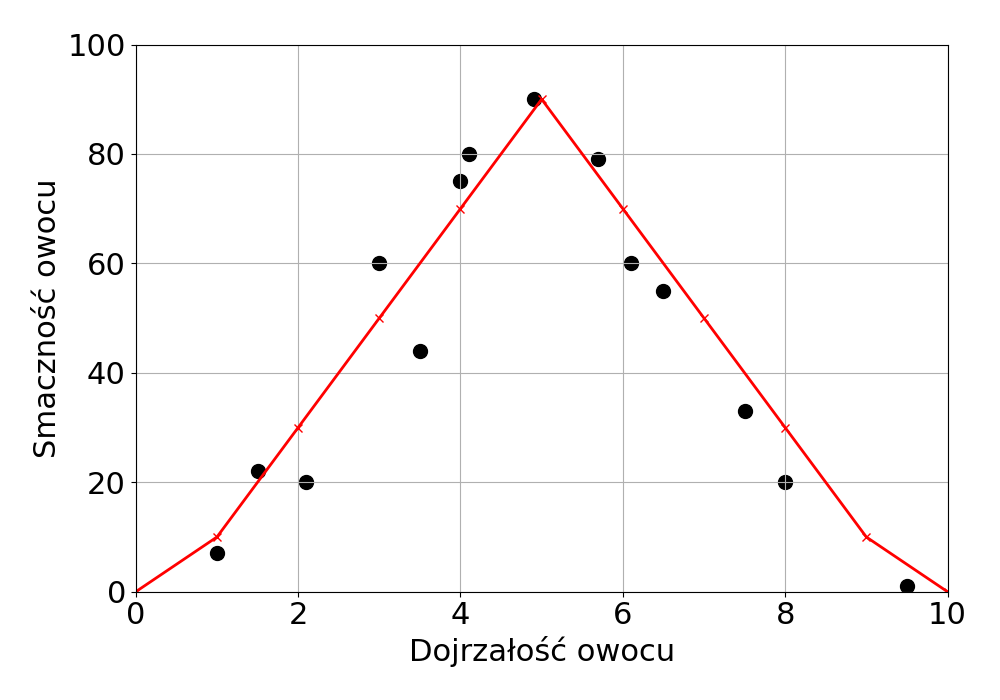
\includegraphics[width=0.6\textwidth]{images/fruit09.png}\end{center}
\end{frame}
\begin{frame}
	\begin{center} $y_{11} = \max(20x - 10, 0)\quad y_{12} = \max(40x - 200, 0)$\\$y_{21} = \max(y_{11} - y_{12}, 0)$ \end{center}
	\begin{center}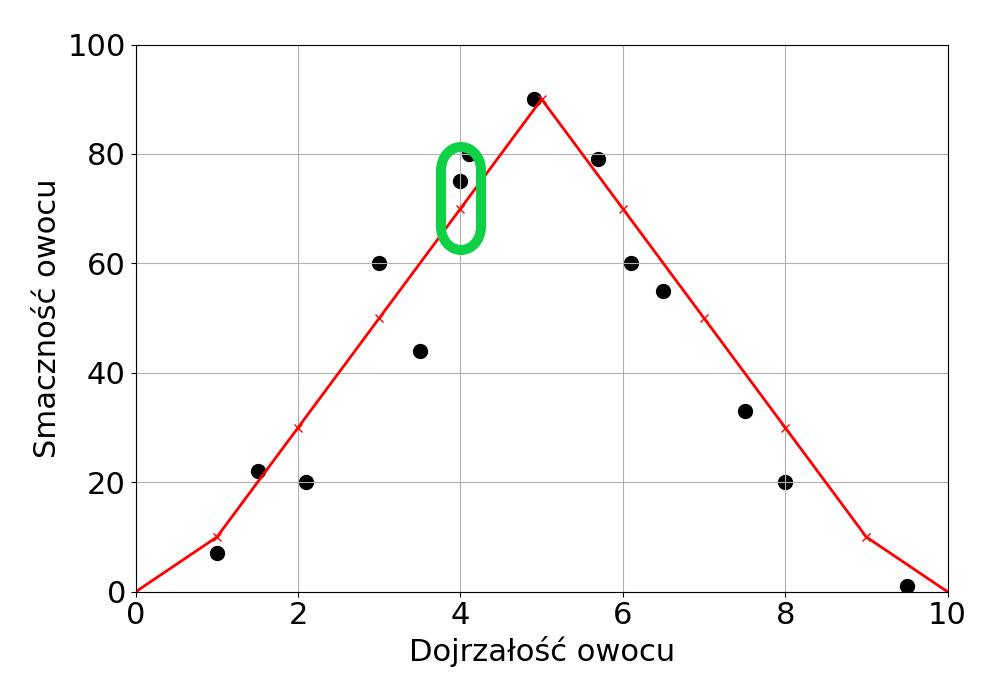
\includegraphics[width=0.6\textwidth]{images/fruit09a.png}\end{center}
\end{frame}
\begin{frame}
	\begin{center}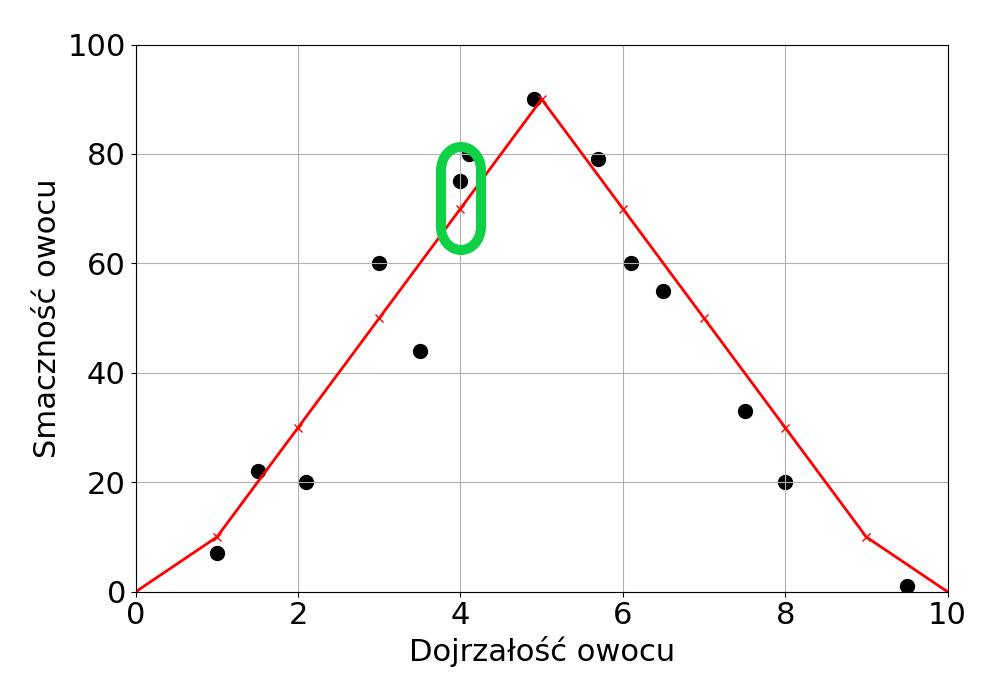
\includegraphics[width=0.3\textwidth]{images/fruit09a.png}\end{center}
	\begin{tabular}{ll}
	$(x = 4, y^{\text{true}} = 75)$ &  \\\pause
	$y_{11} = \max(20\times 4 - 10, 0) = \max(70, 0) = 70$ &  $w_{111}=20, b_{11}=-10$\\\pause
	$y_{12} = \max(40 \times 4 - 200, 0) = \max(-40, 0) = 0$ &  $w_{121} = 40, b_{12}=-200$\\\pause
	$y_{21} = \max(70 - 0, 0) = 70$ 	& $w_{211} = 1, w_{212} = -1, b_{21} = 0$\\\pause
	błąd (loss) $(75 - 70)^2 = 25$ & $L(y^{\text{true}}, y^{\text{out}}) = (y^{\text{true}} - y_{21})^2$\\\pause
	błąd $\sim$ $w_{ijk}$? &
	\end{tabular}
\end{frame}
\begin{frame}
	%\begin{tabular}{l}
	$y_{11} = \max(20x - 10, 0)\quad y_{12} = \max(40x - 200, 0) \quad y_{21} = \max(y_{11} - y_{12}, 0)$ \\\pause 
	
	$y_{11} = \max(z_{11}, 0) \quad z_{11} = w_{111}x + b_{11}$\\
	$y_{12} = \max(z_{12}, 0) \quad z_{12} = w_{121}x + b_{12}$\\
	$y_{21} = \max(z_{21}, 0) \quad z_{21} = w_{211}y_{11} + w_{212}y_{12} + b_{21}$\vskip 0.3 cm\pause

	$\frac{\partial L}{\partial y_{21}} = \frac{\partial }{\partial y_{21}} (y^{\text{true}^2} - 2y^{\text{true}}y_{21} + y_{21}^2) = 2y_{21} - 2y^{\text{true}}$\vskip 0.3 cm\pause
	$\frac{\partial L}{\partial z_{21}} = \frac{\partial L}{\partial y_{21}}\frac{\partial y_{21}}{\partial z_{21}} \quad \frac{\partial y_{21}}{\partial z_{21}} = \{0\:\text{if}\: z_{21} < 0; 1\:\text{if}\: z_{21} > 0 \}$\vskip 0.3 cm
	(Reguła łańcuchowa $\frac{\partial L}{\partial w} = \frac{\partial L}{\partial y} \frac{\partial y}{\partial z} \frac{\partial z}{\partial w}$)\vskip 0.3 cm\pause
	
	$\frac{\partial L}{\partial w_{211}} =  \frac{\partial L}{\partial y_{21}}\frac{\partial y_{21}}{\partial z_{21}}\frac{\partial z_{21}}{\partial w_{211}}  \quad  \frac{\partial z_{21}}{\partial w_{211}} = y_{11}$\\\pause
	\dots \\\pause
	$\frac{\partial L}{\partial w_{ijk}}$ (zależność błędu od wagi)\vskip 0.3 cm\pause
	$\Delta w_{ijk} = - \gamma \frac{\partial L}{\partial w_{ijk}}$ (aktualizacja wagi)
	%\end{tabular}
\end{frame}
\begin{frame}
	\begin{enumerate}
		\item Sieć neuronowa: wagi (+bias, architektura)
		\item Przykład (sample) i wartość wymagana dla niego (ground truth)
		\item Wyliczenie wartości częściowych i końcowych dla przykładu (forward pass)
		\item Miara błędu (loss)
		\item Wsteczna propagacja błędu (backpropagation) -- wyznaczenie gradientów
		\item Aktualizacja wag sieci
	\end{enumerate}
\end{frame}

\subsection{[Stochastic] gradient descent}

\begin{frame}
	Mamy:
	\begin{enumerate}
		\item Adaptacja (aktualizacja) wag dla konkretnego przykładu (punktu danych)
	\end{enumerate}\pause
	Dalsze zagadnienia:
	\begin{enumerate}
		\item Wiele punktów danych -- optymalizacja
		\item Model danych i skuteczna predykcja z modelu
		\item Współczynnik szybkości uczenia (learning rate), zanikające i eksplodujące gradienty, zagadnienia optymalizacji, inicjalizacja, \dots
	\end{enumerate}
\end{frame}
\begin{frame}
	,,Gradient prosty'' (gradient descent):
	\begin{enumerate}
		\item Mamy $\frac{\partial L}{\partial w_{ijk}}$
		\item Minimalizujemy $L$ -- błąd zmniejsza się najszybciej jeżeli idziemy w kierunku przeciwnym do gradientu
		\item Iteracyjnie modyfikujemy wagi $w_{ijk}^{n+1} = w_{ijk}^{n} - \gamma \frac{\partial L}{\partial w_{ijk}}$
		\item Zejdziemy wzdłuż gradientu do zera i problem rozwiązany?\pause\ Niestety, bardziej skomplikowane\dots
		\item Na początek -- jak wyliczyć gradient -- mamy $m=12$ przykładów
	\end{enumerate}
	\begin{tabular}{lll}
	\newmoon\newmoon\newmoon\newmoon\newmoon\newmoon\newmoon\newmoon\newmoon\newmoon\newmoon\newmoon & (wykorzystujemy wszystkie) & batch gradient descent\\
	\fullmoon\newmoon\fullmoon\fullmoon\fullmoon\fullmoon\fullmoon\fullmoon\fullmoon\fullmoon\fullmoon\fullmoon & (wykorzystujemy jeden) & stochastic gradient descent\\
    \fullmoon\fullmoon\fullmoon\fullmoon\newmoon\newmoon\newmoon\newmoon\fullmoon\fullmoon\fullmoon\fullmoon & (wykorzystujemy podzbiór) & minibatch gradient descent
	\end{tabular}
\end{frame}
\begin{frame}
	\begin{enumerate}
		\item Gradient descent -- iteracyjne poprawianie sieci % często  stochastic == minibatch
			\begin{enumerate}
				\item \textbf{batch gradient descent }-- aktualizacja modelu dopiero po przejściu przez wszystkie przykłady treningowe -- kosztowne obliczeniowo i pamięciowo
				\item \textbf{stochastic gradient descent} -- aktualizacja modelu po analizie pojedynczego przykładu -- mniejsze wymagania obliczeniowe i pamięciowe, mogą pojawić się fluktuacje błędu
				\item \textbf{minibatch gradient descent} -- praktyczny kompromis
			\end{enumerate}
		\item Przejście przez wszystkie przykłady zbioru treningowego -- epoka (\textbf{epoch})\pause
		\item Przygody na szlaku z gradientem\pause
			\begin{enumerate}
				\item Lokalne minima (\textbf{local minima})\pause
				\item Punkt siodłowy (\textbf{saddle point})\pause
				\item Zanikający gradient (\textbf{vanishing gradient})\pause
				\item Eksplodujący gradient (\textbf{exploding gradient})\pause
			\end{enumerate}
	\end{enumerate}
\end{frame}
\begin{frame}
	\begin{columns}[onlytextwidth]
		\begin{column}{.4\textwidth}
			\begin{figure}
				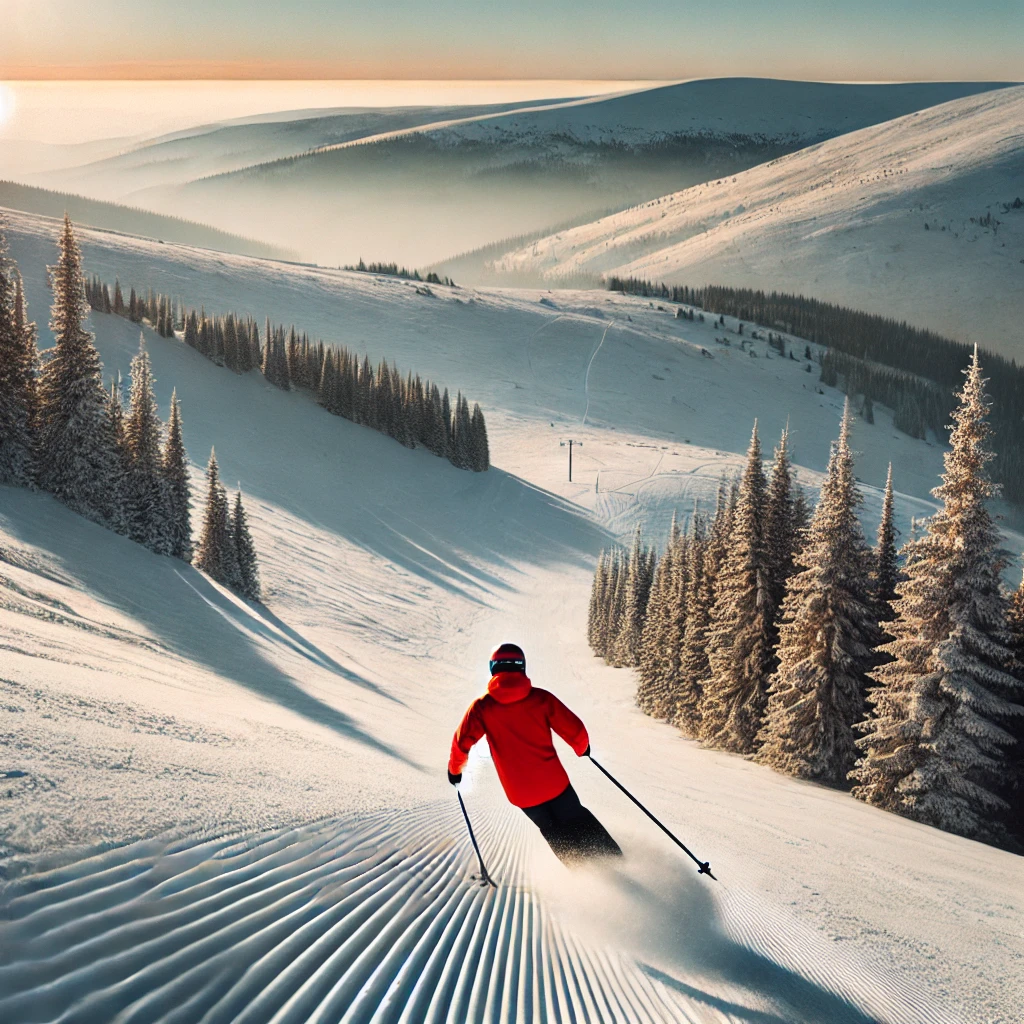
\includegraphics[width=\textwidth]{images/nice.png}
				\caption{Gradient descent w typowych ilustracjach}
			\end{figure}
		\end{column}
		%\hfill
		\pause
		\begin{column}{.4\textwidth}
			\begin{figure}
				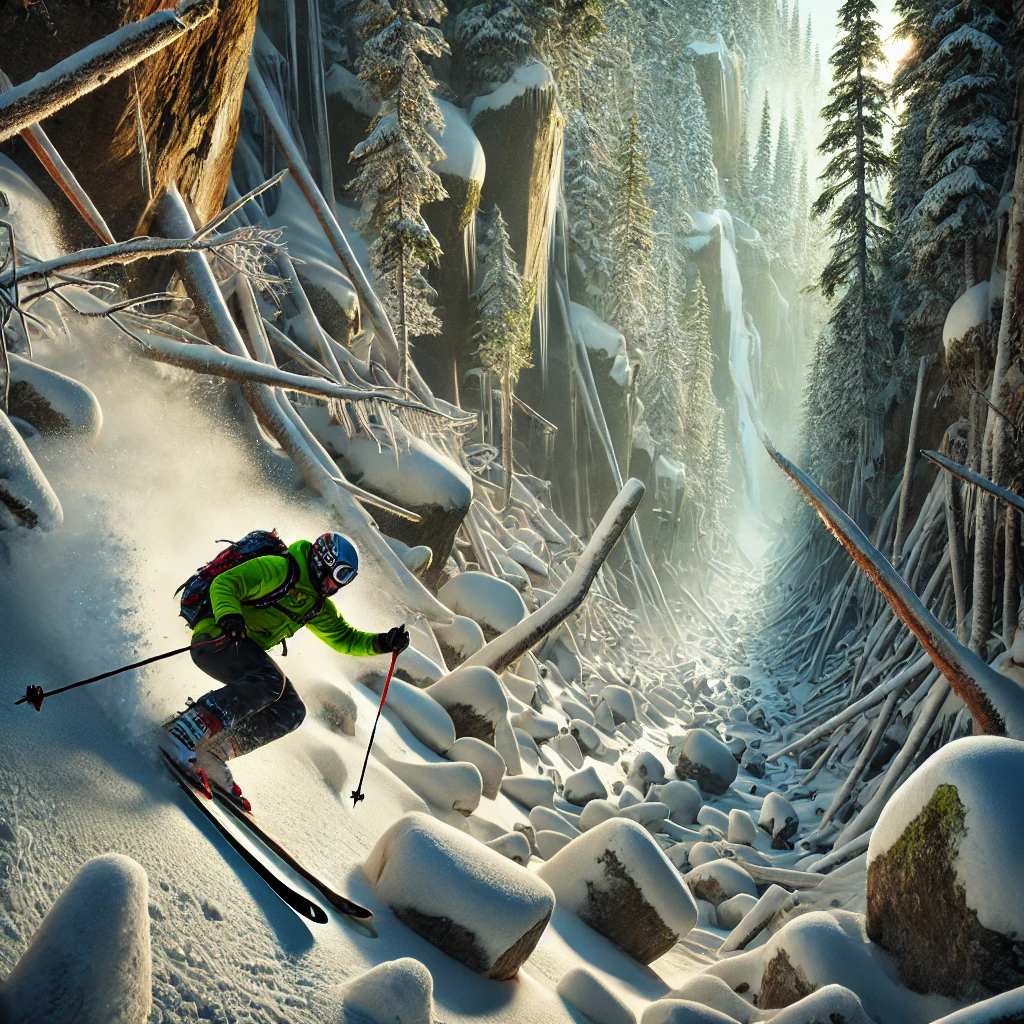
\includegraphics[width=\textwidth]{images/notnice2.png}
				\caption{Gradient descent w praktyce}
			\end{figure}
		\end{column}
	\end{columns}
	\centering{\tiny źródło ilustracji:DALL$\cdot$E}
\end{frame}

\subsection{Learning rate}

\begin{frame}
	Mamy:
	\begin{enumerate}
		\item Adaptacja (aktualizacja) wag dla konkretnego przykładu (punktu danych)
		\item Optymalizacja -- iteracyjne przejście przez kolejne punkty danych i modyfikacje wag
	\end{enumerate}\pause
	Dalsze zagadnienia:
	\begin{enumerate}
		\item Krzywa błędu (\textbf{loss curve})
		\item Learning rate
		\item Optymalizacja++
	\end{enumerate}
\end{frame}
\begin{frame}
	\begin{columns}[onlytextwidth]
	\begin{column}{.3\textwidth}
		\begin{figure}
			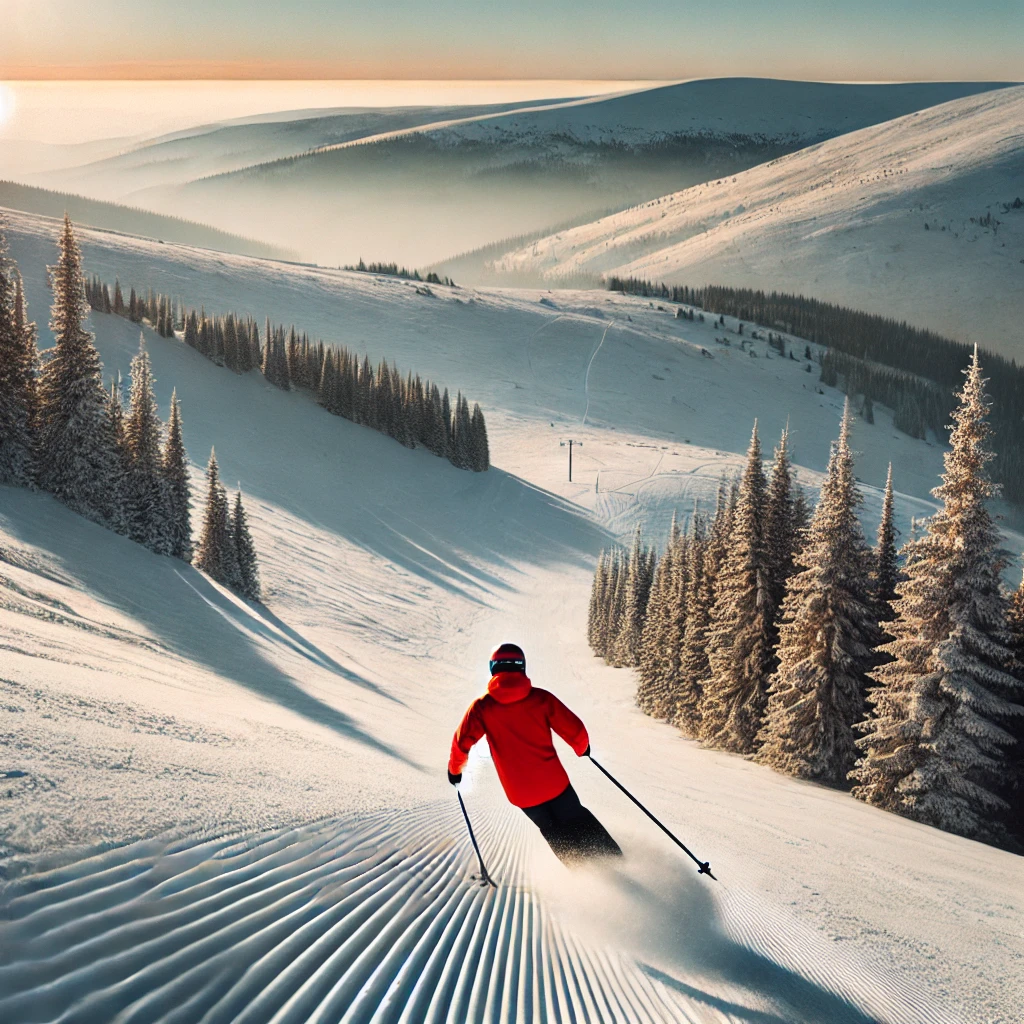
\includegraphics[width=\textwidth]{images/nice.png}
		\end{figure}
	\end{column}
	%\hfill
	\begin{column}{.6\textwidth}
		\begin{figure}
			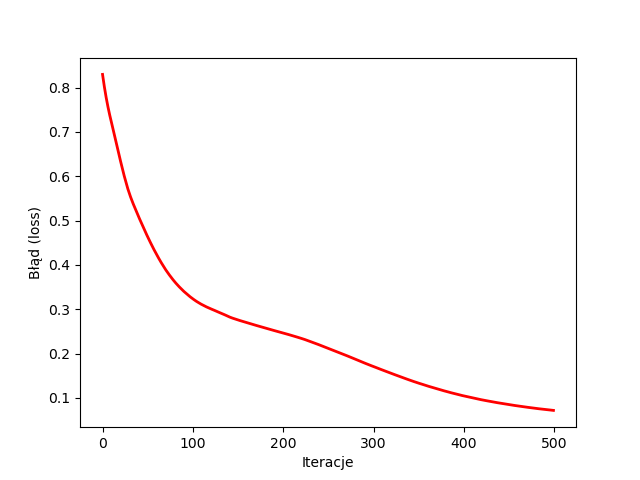
\includegraphics[width=\textwidth]{images/loss.png}
			\caption{Przykładowa krzywa błędu}
		\end{figure}
	\end{column}
	\end{columns}
\end{frame}
\begin{frame}
	\begin{columns}[onlytextwidth]
		\begin{column}{.3\textwidth}
			\begin{figure}
				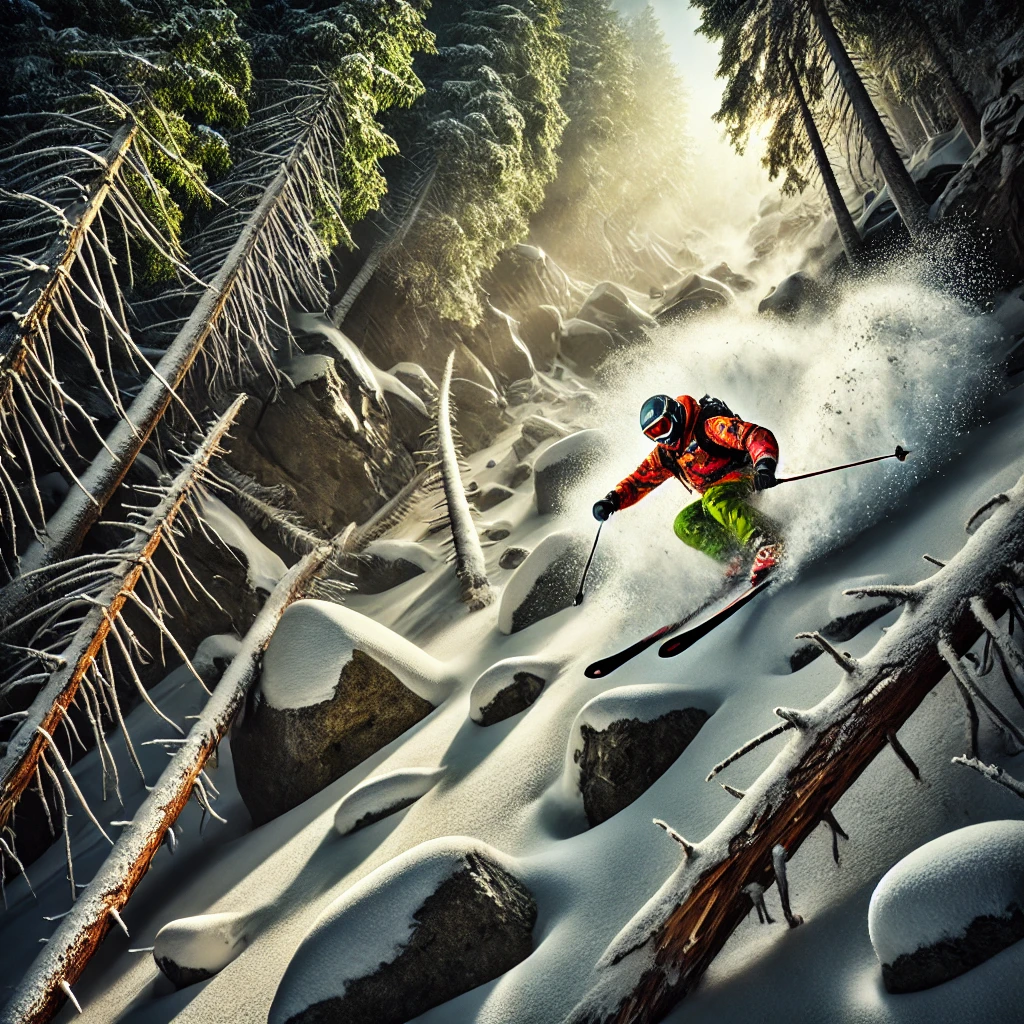
\includegraphics[width=\textwidth]{images/notnice.png}
			\end{figure}
		\end{column}
		%\hfill
		\begin{column}{.6\textwidth}
			\begin{figure}
				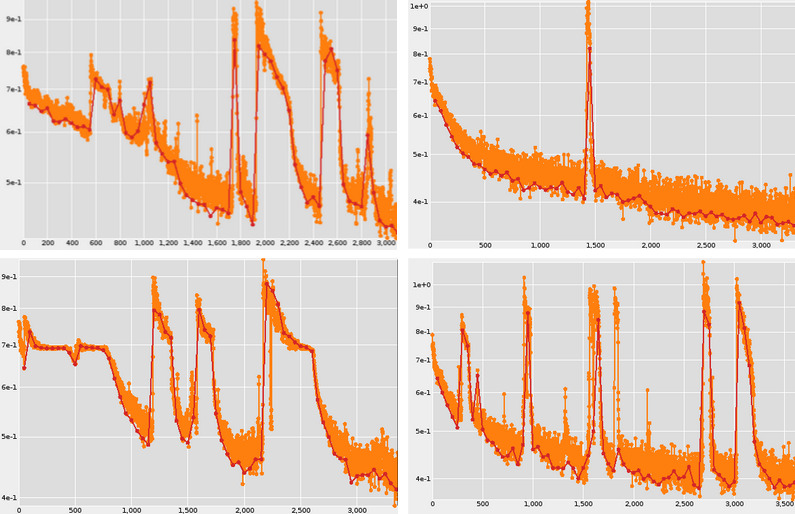
\includegraphics[width=\textwidth]{images/tumblr_nu1yzl1ss61ue62ito1_1280.jpg}
				\caption{\emph{Taming Spatial Transformer Networks, contributed by Diogo. For the record, it’s not supposed to look like that.} (Pobrane z \url{https://lossfunctions.tumblr.com/})}
			\end{figure}
		\end{column}
	\end{columns}
\end{frame}
\begin{frame}
	\begin{columns}[onlytextwidth]
		\begin{column}{.3\textwidth}
			\begin{figure}
				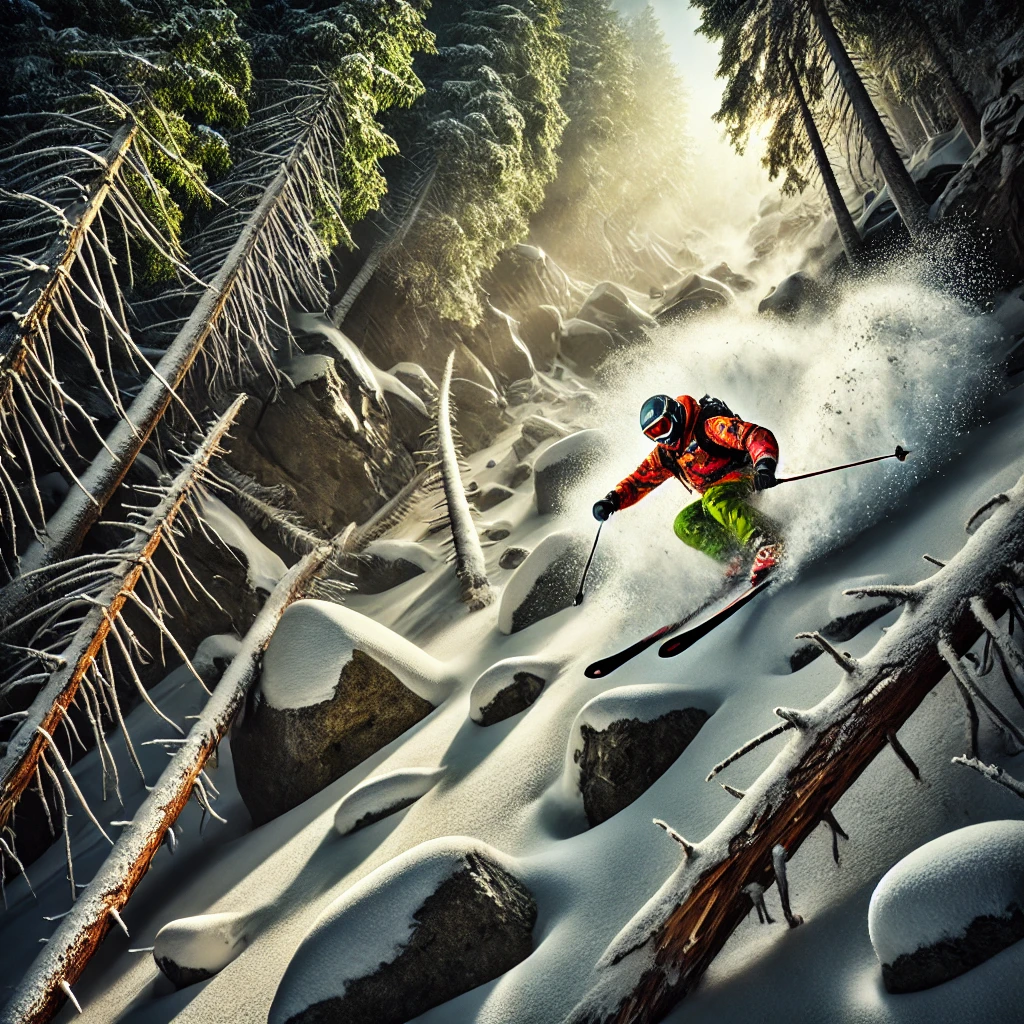
\includegraphics[width=\textwidth]{images/notnice.png}
			\end{figure}
		\end{column}
		%\hfill
		\begin{column}{.6\textwidth}
			\begin{figure}
				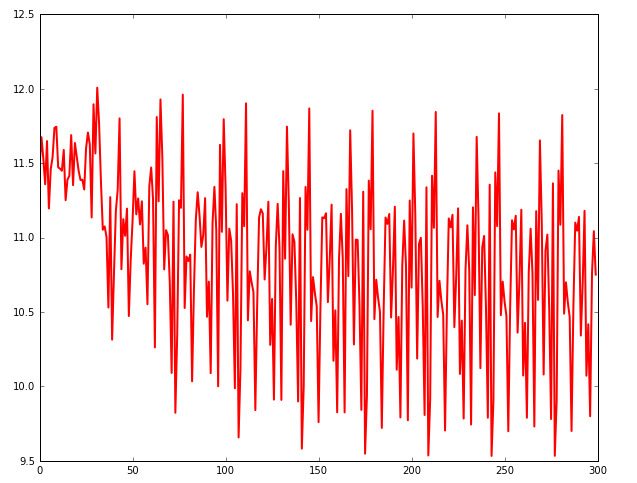
\includegraphics[width=0.7\textwidth]{images/tumblr_ofkdzjlKui1ue62ito1_640.jpg}
				\caption{\emph{A heart rate or a loss function? :)
						
						This one of a custom implementation of an RNN, graciously contributed by Ray Zhang.
					} (Pobrane z \url{https://lossfunctions.tumblr.com/})}
			\end{figure}
		\end{column}
	\end{columns}
\end{frame}
\begin{frame}
	\begin{columns}[onlytextwidth]
		\begin{column}{.3\textwidth}
			\begin{figure}
				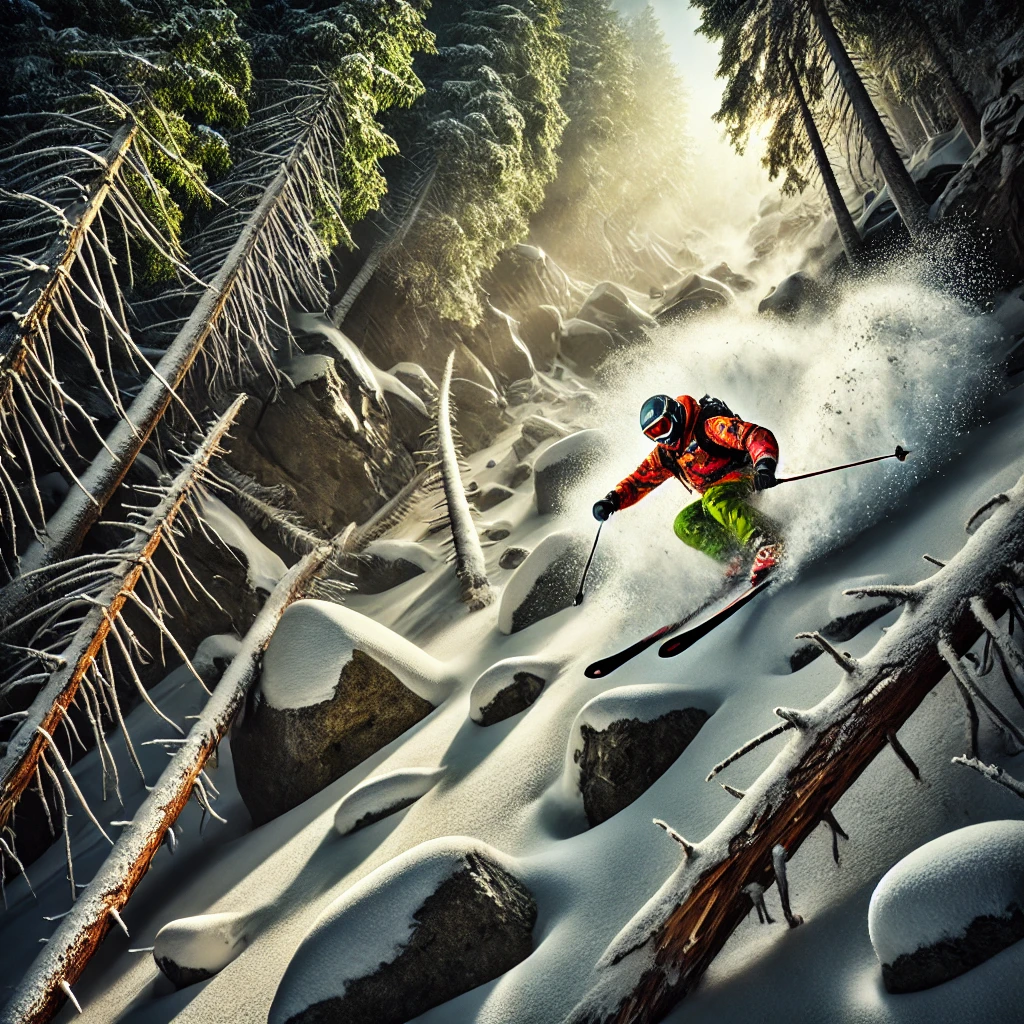
\includegraphics[width=\textwidth]{images/notnice.png}
			\end{figure}
		\end{column}
		%\hfill
		\begin{column}{.6\textwidth}
			\begin{figure}
				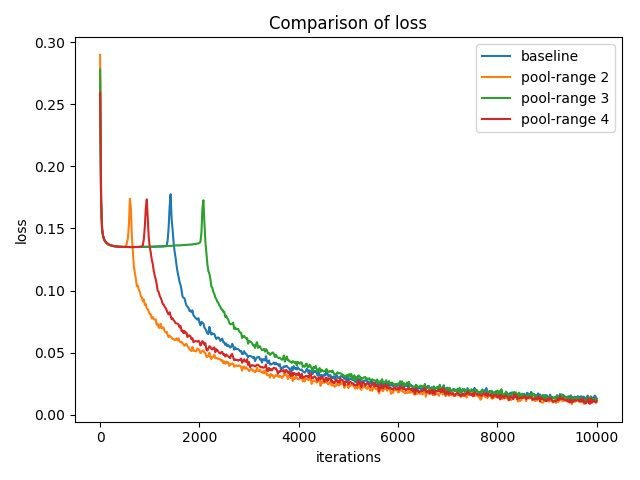
\includegraphics[width=0.8\textwidth]{images/tumblr_p0x789Ry1y1ue62ito1_640.jpg}
				\caption{\emph{A highly amusing specimen from @\_karfly . Truly baffles the mind.} (Pobrane z \url{https://lossfunctions.tumblr.com/})}
			\end{figure}
		\end{column}
	\end{columns}
\end{frame}
\begin{frame}
	\begin{columns}[onlytextwidth]
	\begin{column}{.3\textwidth}
		\begin{figure}
			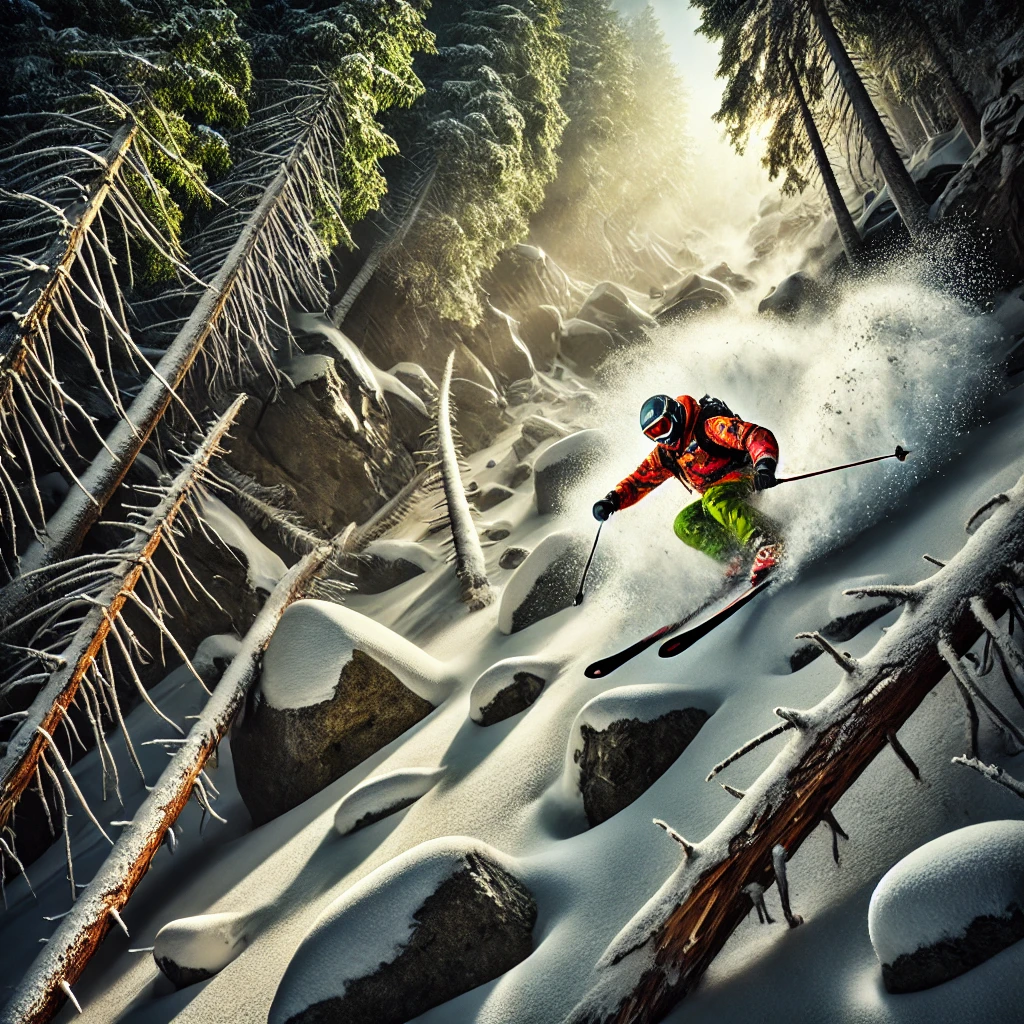
\includegraphics[width=\textwidth]{images/notnice.png}
		\end{figure}
	\end{column}
	%\hfill
	\begin{column}{.65\textwidth}
		\begin{center}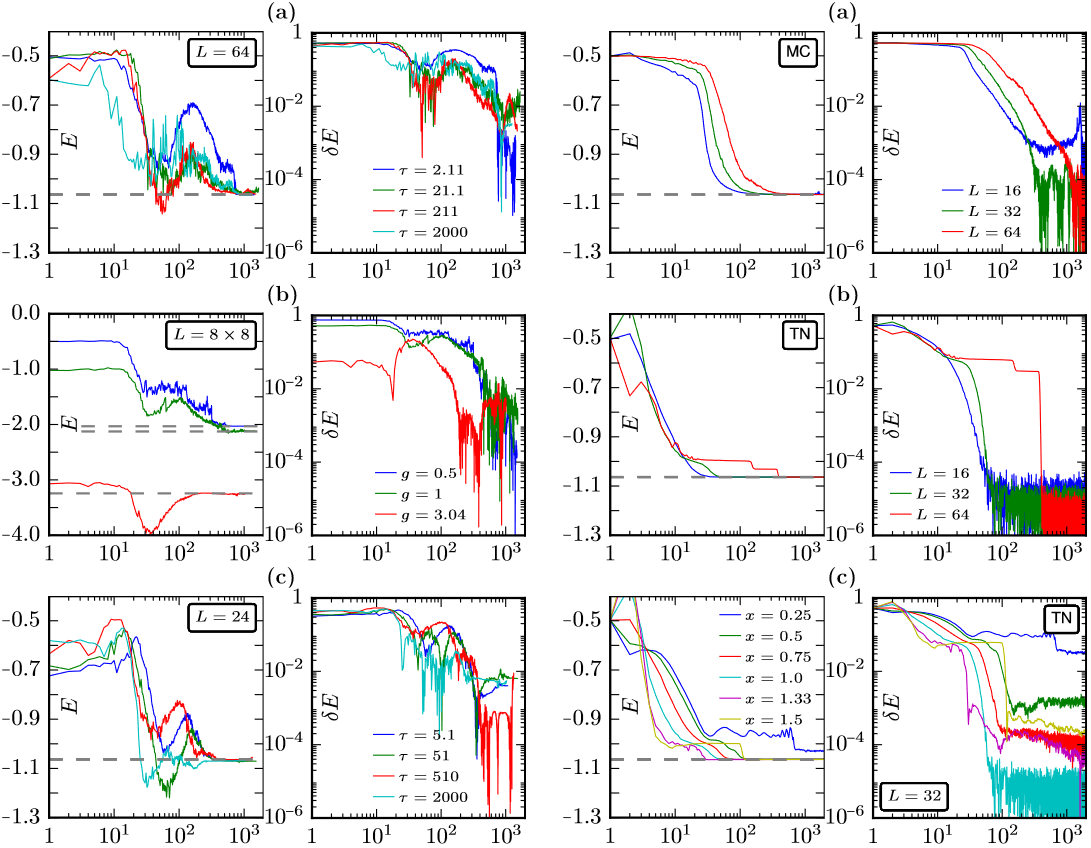
\includegraphics[width=0.9\textwidth]{images/qenergy.png}\end{center}
	{\tiny B. Gardas et al, Quantum neural networks to simulate many-body quantum systems, Phys. Rev. B 98, 184304 (2018)}
	\end{column}
	\end{columns}
\end{frame}
\begin{frame}
	
	{\footnotesize
	\emph{	redback.bjfu.ws: Why is my loss function going down and jumping?\\
		J\_Johnson: It’s not always a straight path to the best fit. In fact, usually it’s pretty bumpy. }\\
	(z: \url{https://discuss.pytorch.org/t/why-is-my-loss-function-going-down-and-jumping/170508})
	}
	\vskip 0.5 cm
	
	Kontrola procesu treningu:
	\begin{enumerate}
		\item Współczynnik szybkości uczenia (\textbf{learning rate}) $\gamma$, $w_{ijk}^{n+1} = w_{ijk}^{n} - \textcolor{red}{\gamma} \frac{\partial L}{\partial w_{ijk}}$
	\end{enumerate}
\end{frame}

\begin{frame}
	Learning rate:
	\begin{itemize}
		\item Typowe wartości $0.1 - 0.001$
		\item Zbyt niskie wartości (zwykle) -- wydłużony czas uczenia; wysokie -- zatrzymanie uczenia, oscylacje
		\item Algorytmy: np. Adagrad, RMSprop, Adam\dots
	\end{itemize}
	\begin{center}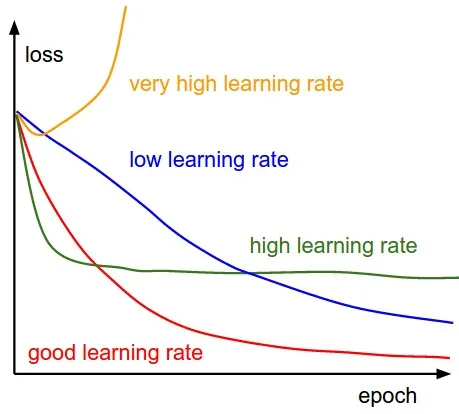
\includegraphics[width=0.3\textwidth]{images/lr.png}\end{center}
	{\tiny Źródło ilustracji: \href{http://cs231n.github.io/assets/nn3/learningrates.jpeg}{CS231n Convolutional Neural Networks for Visual Recognition}}
\end{frame}

\begin{frame}
	\begin{itemize}
		\item Algorytmy: np. Adagrad, RMSprop, Adam\dots
			\begin{itemize}
				\item Pęd gradientu (\textbf{momentum}) -- przejście przez punkty siodłowe (gdzie gradient ma niewielkie wartości) i lokalne minima \\
				 $v^{n} = \mu v^{n-1} - \gamma \frac{\partial L}{\partial w_{ijk}}\qquad w_{ijk}^{n+1} = w_{ijk}^{n} + v^{n}$
				\item Skalowanie (\textbf{learning rate annealing/decay}), np. $\gamma_n = \gamma_0e^{-dn}$ -- zmniejszanie wartości w trakcie uczenia
			\end{itemize}
	\end{itemize}
\end{frame}

\begin{frame}
	
	{\footnotesize
		\emph{	redback.bjfu.ws: Why is my loss function going down and jumping?\\
			J\_Johnson: It’s not always a straight path to the best fit. In fact, usually it’s pretty bumpy. }\\
		(z: \url{https://discuss.pytorch.org/t/why-is-my-loss-function-going-down-and-jumping/170508})
	}
	\vskip 0.5 cm
	
	Kontrola procesu treningu:
	\begin{enumerate}
		\item Współczynnik szybkości uczenia (\textbf{learning rate}) $\gamma$, $w_{ijk}^{n+1} = w_{ijk}^{n} - \textcolor{red}{\gamma} \frac{\partial L}{\partial w_{ijk}}$
		\item Rozmiar podzbioru danych (\textbf{batch size})
	\end{enumerate}
\end{frame}

\begin{frame}
	Batch size (BS):\\
	\begin{tabular}{ll}
	\st{\newmoon\newmoon\newmoon\newmoon\newmoon\newmoon\newmoon\newmoon\newmoon\newmoon\newmoon\newmoon} & (niepraktyczne)\\
	\fullmoon\newmoon\fullmoon\fullmoon\fullmoon\fullmoon\fullmoon\fullmoon\fullmoon\fullmoon\fullmoon\fullmoon & \\
	\fullmoon\fullmoon\fullmoon\fullmoon\fullmoon\fullmoon\fullmoon\fullmoon\newmoon\newmoon\fullmoon\fullmoon & \\
	\fullmoon\fullmoon\fullmoon\fullmoon\newmoon\newmoon\newmoon\newmoon\fullmoon\fullmoon\fullmoon\fullmoon & 
	\end{tabular}
	\vskip 0.3cm
	\begin{description}
		\item[popularne wartości] np. 32, 64 / 128, 256
		\item[małe wartości] np. 1, 2, 4, 8 -- szybsze zmiany w sieci (więcej na epokę)%potencjalnie lepsze wyniki, ale wymaga więcej czasu i zasobów obliczeniowych
		\item[duże wartości] wymagają więcej pamięci, mniej szumu
	\end{description}
	\vskip 0.3cm
	Przy małej wartości BS mogą pojawić się fluktuacje (widoczne w krzywej błędu), niekoniecznie negatywne -- mogą uodparniać przed przetrenowaniem
	%Large batch sizes can lead to faster training times but may result in lower accuracy and overfitting, 
	% data, while larger batch sizes are more resistant to these fluctuations but may converge more slowly.
	%Small batch sizes can be more susceptible to random fluctuations in the training 
\end{frame}

\begin{frame}
	Stochastic vs minibatch vs batch gradient descent
	\begin{center}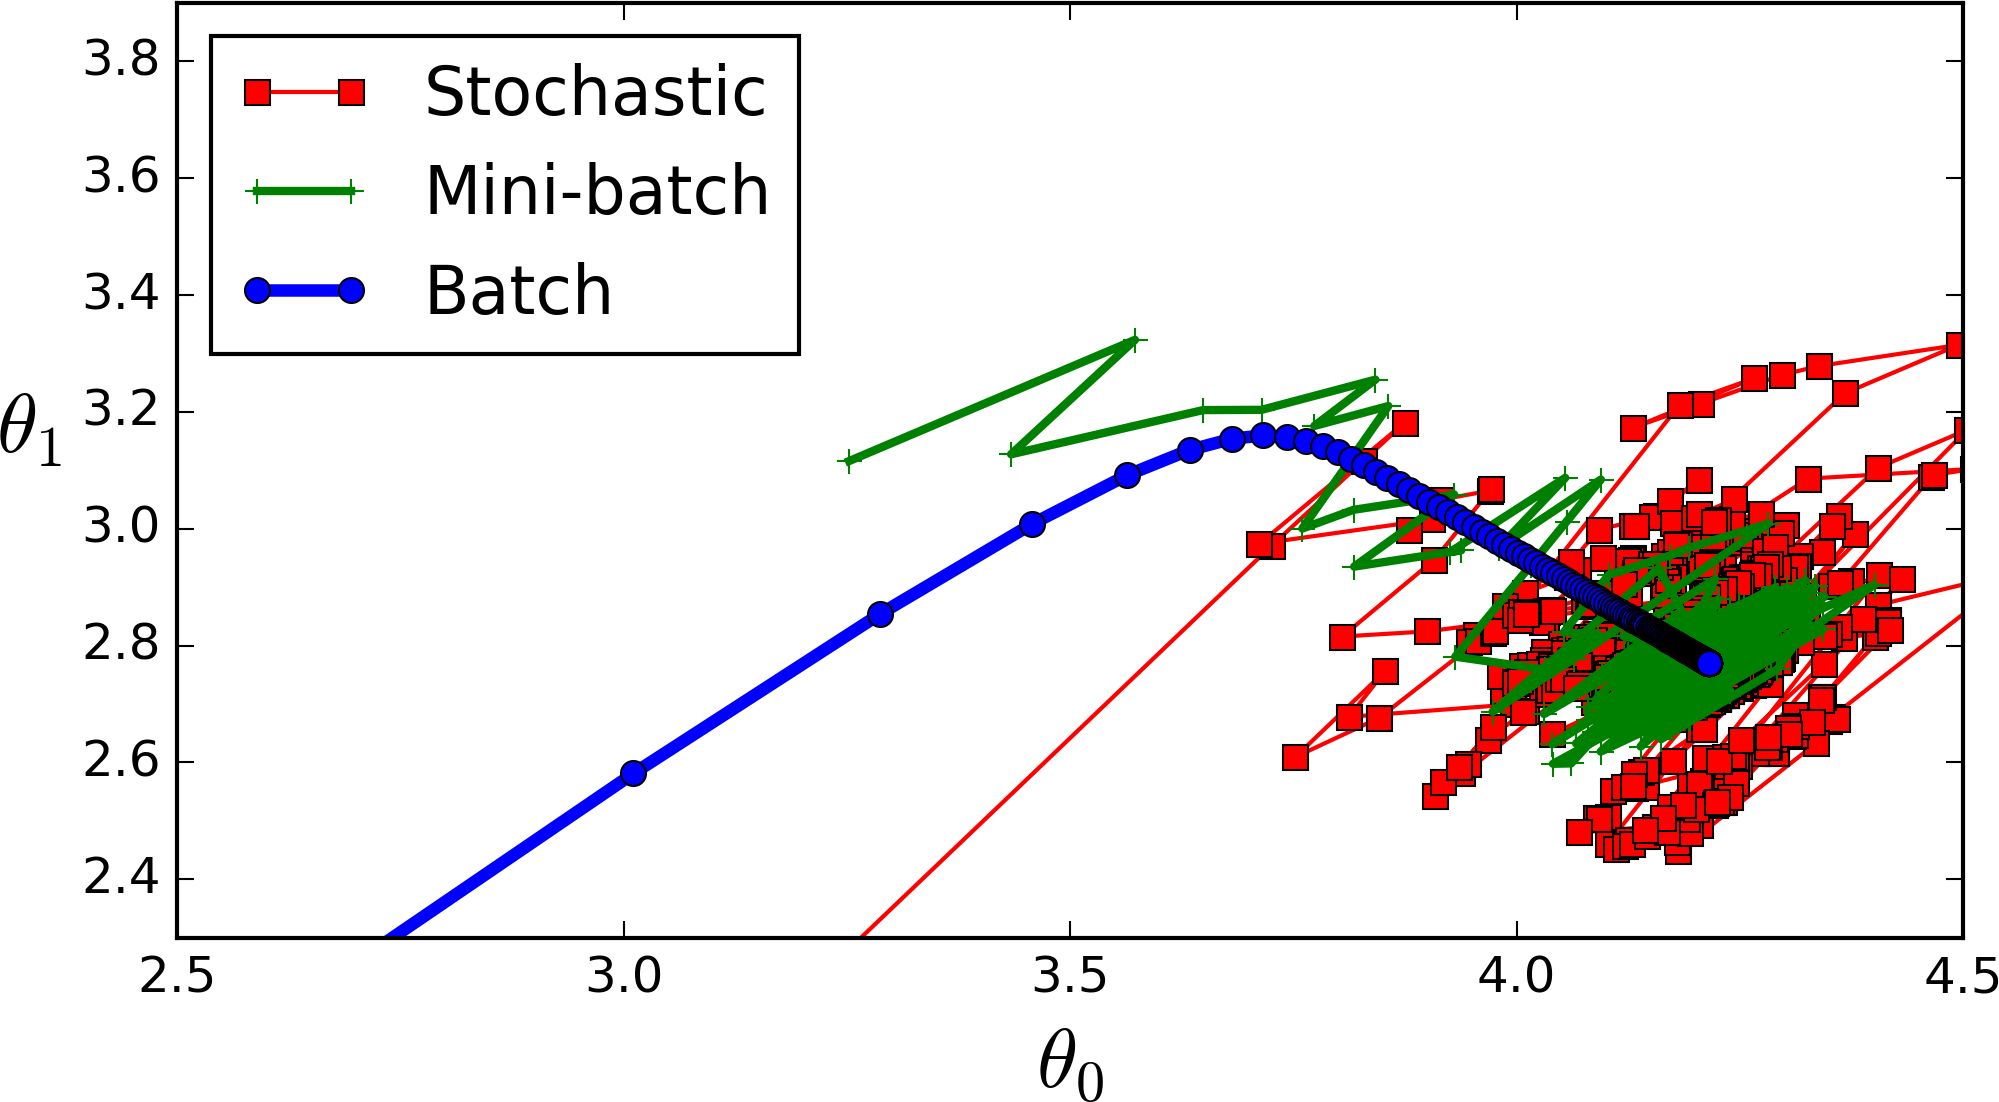
\includegraphics[width=0.67\textwidth]{images/lU3sx.png}\end{center}
	{\tiny Źródło ilustracji: \href{https://stats.stackexchange.com/questions/153531/what-is-batch-size-in-neural-network}{Odpowiedź \emph{itdxer} w pytaniu \emph{What is batch size in neural network?} CrossValidated StackExchange}}
\end{frame}


\subsection{Wartości gradientu, inicjalizacja -- wartości początkowe}


\begin{frame}
	$y_{11} = \max(20x - 10, 0)$\\\pause 
	$y_{21} = \max(20y_{11} - 10, 0)\quad y_{31} = \max(20y_{21} - 10, 0) \quad y_{41} = \max(20y_{31} - 10, 0)$\\\pause 
	$x = 1 \rightarrow y_{11} = 10 \quad y_{21} = 190 \quad y_{31} = 3790 \quad y_{41} = 75790$\vskip 0.5 cm\pause 
	$y_{11} = \max(0.2x, 0) \quad  y_{21} = \max(0.2y_{11}, 0) \quad \dots $\\\pause 
	$x = 1 \rightarrow y_{11} = 0.2 \quad y_{21} = 0.04 \quad y_{31} = 0.008 \quad y_{41} = 0.0016$\vskip 0.5 cm\pause 
	\begin{itemize}
		\item Wartości ,,przepływają'' przez sieć, podczas wyliczania wyjść neuronów ($\rightarrow$) i gradientów~($\leftarrow$)
		\item Wartości wyliczanych wyjść/gradientów wrażliwe na zakres wartości wag
		\item Eksplodujący gradient (\textbf{exploding gradients}) -- duże modyfikacje do wag, niestabilności/NaN
		\item Zanikający gradient (\textbf{vanishing gradient}) -- małe (lub brak) modyfikacji do wag, spowolniony/zatrzymany proces uczenia
	\end{itemize}
\end{frame}

\begin{frame}
	\begin{enumerate}
		\item Przygotowanie danych
			\begin{description}
				\item[Normalizacja] kontrola zakresu danych, np. $\hat{x}_{ij} = \frac{x_{ij} - \min \mathbf{x}_{i}}{\max \mathbf{x}_{i} - \min \mathbf{x}_{i}}$
				\item[Standaryzacja] korekta względem średniej i wariancji $\hat{x}_{ij} = \frac{x_{ij} - \mu_i}{\sigma_i}$
			\end{description}\pause
		\item Przygotowanie sieci
			\begin{description}
				\item[Inicjalizacja] początkowe wartości wag losowane np. $w_{ijk} = \mathcal{N}(\mu=0,\sigma=0.01)$
				\item[Xavier Glorot] uwzględnia średnią liczbę połączeń do neuronu $w_{ijk} = \mathcal{N}\left(\mu=0,\sigma=\sqrt{\frac{1}{\mathrm{fan_{avg}}}}\right)$ lub $w_{ijk} = \mathcal{U}\left(\sqrt{\frac{3}{\mathrm{fan_{avg}}}}\right)$
				\item[Kaming He] rozwija inicjalizację XG pod kątem ReLU $w_{ijk} = \mathcal{N}\left(\mu=0,\sigma=\sqrt{\frac{2}{\mathrm{fan_{in}}}}\right)$ lub $w_{ijk} = \mathcal{U}\left(\sqrt{\frac{6}{\mathrm{fan_{avg}}}}\right)$
			\end{description}\pause
		\item Losowa inicjalizacja + optymalizacja lokalna = możliwe różne wyniki treningu w zależności od stanu początkowego 		
	\end{enumerate}
\end{frame}


\subsection{Regularyzacja}


\begin{frame}
	\begin{itemize}
		\item Wsparcie treningu -- kontrola wartości wag
		\begin{description}
			%Dropout:%Randomly deactivating neurons during training introduces noise that can help escape local minima and promotes generalization.
			\item[Dropout] z określonym prawdopodobieństwem (np. $p=0.2$ albo $p=0.5$) zerujemy wyjście z neuronu w trakcie treningu\\
			\begin{center}
\includegraphics[width=0.2\textwidth]{images/drop0.png}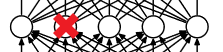
\includegraphics[width=0.2\textwidth]{images/drop1.png}
\includegraphics[width=0.2\textwidth]{images/drop2.png}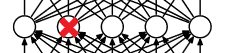
\includegraphics[width=0.2\textwidth]{images/drop3.png}\end{center}\pause
			\item[Batch Normalization] normalizacja i przeskalowanie wartości pomiędzy warstwami $y = \gamma \frac{x - \mu_{B}}{\sigma_B} + \beta$ (standaryzacja + przeskalowanie + przesunięcie)\pause
			\item[L2/L1 regularization] ,,kara'' dla wysokich wartości wag\\
			$L(y^{\text{true}}, y^{\text{out}}) = (y^{\text{true}} - y_{21})^2 + \textcolor{red}{\lambda \sum_{i=1}^n w_i^2}$\\
			$L(y^{\text{true}}, y^{\text{out}}) = (y^{\text{true}} - y_{21})^2 + \textcolor{red}{\lambda \sum_{i=1}^n|w_i|}$
		\end{description}
	\end{itemize}
\end{frame}
%Weight Decay (L2 Regularization):%Prevents the model from overfitting and constraining the weights may smooth the loss landscape.


\begin{frame}
	Mamy:
	\begin{enumerate}
		\item Adaptacja (aktualizacja) wag dla konkretnego przykładu (punktu danych)
		\item Optymalizacja -- iteracyjne przejście przez kolejne punkty danych i modyfikacje wag
		\item Sterowanie procesem uczenia -- learning rate, batch size, wybór optymalizatora
		\item Inicjalizacja
		\item Regularyzacja
	\end{enumerate}
\end{frame}


\subsection{Zbiory testowe, walidacyjne, przetrenowanie, hiperparametry}


\newcommand{\thiscaly}{0.9}

\begin{frame}\begin{center}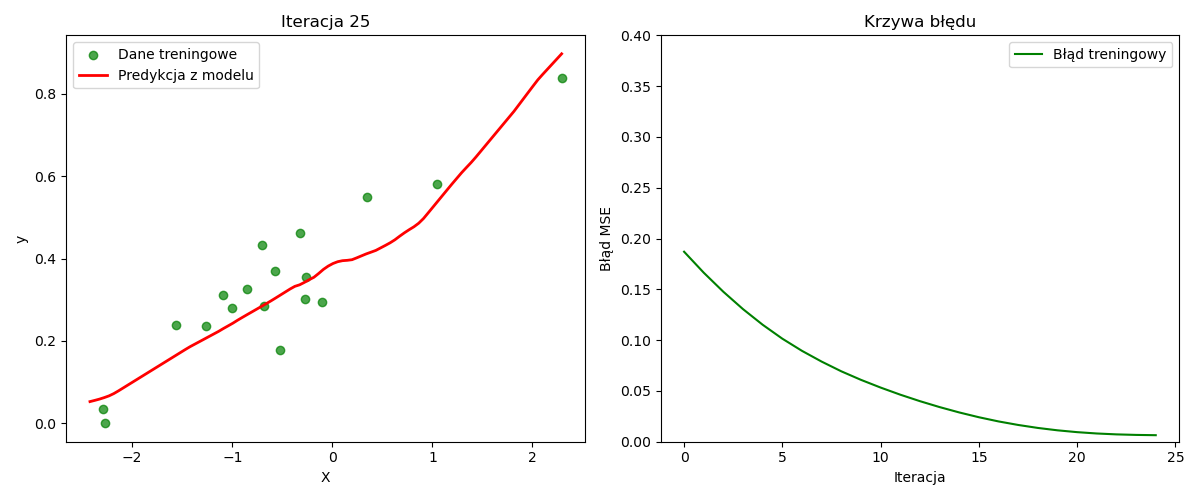
\includegraphics[width=\thiscaly\textwidth]{images/ot25False.png}\end{center}\end{frame}
\begin{frame}\begin{center}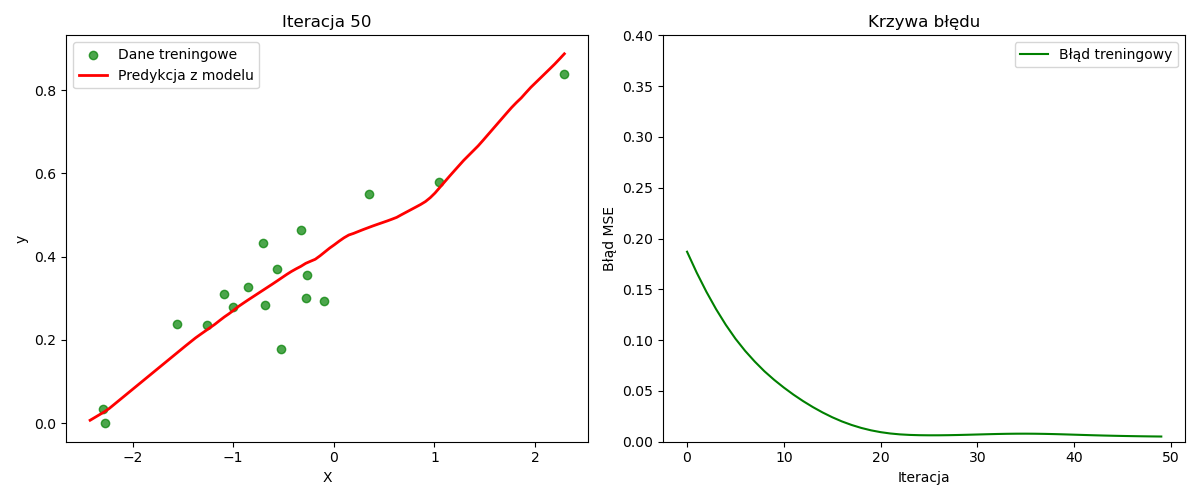
\includegraphics[width=\thiscaly\textwidth]{images/ot50False.png}\end{center}\end{frame}
\begin{frame}\begin{center}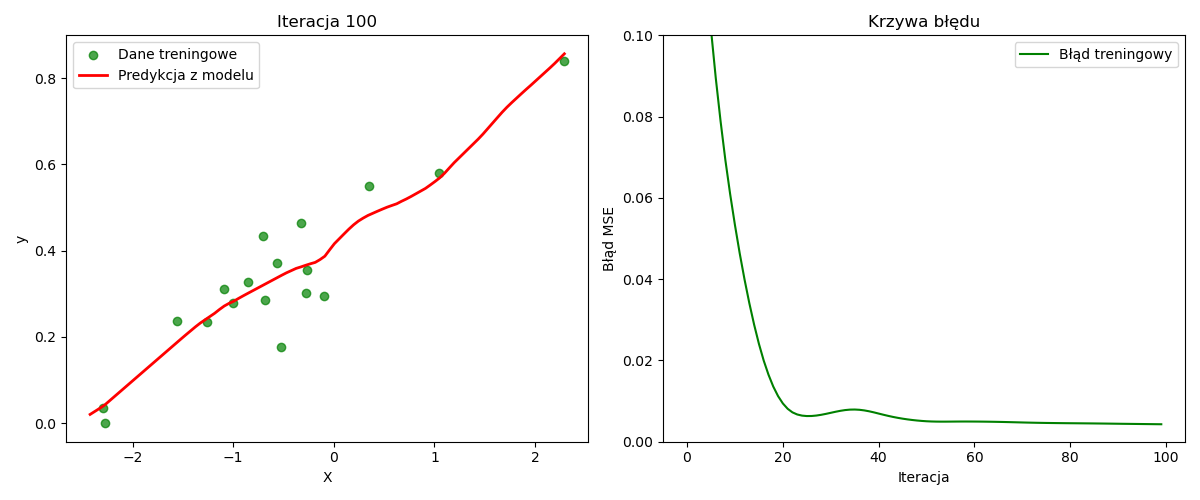
\includegraphics[width=\thiscaly\textwidth]{images/ot100False.png}\end{center}\end{frame}
\begin{frame}\begin{center}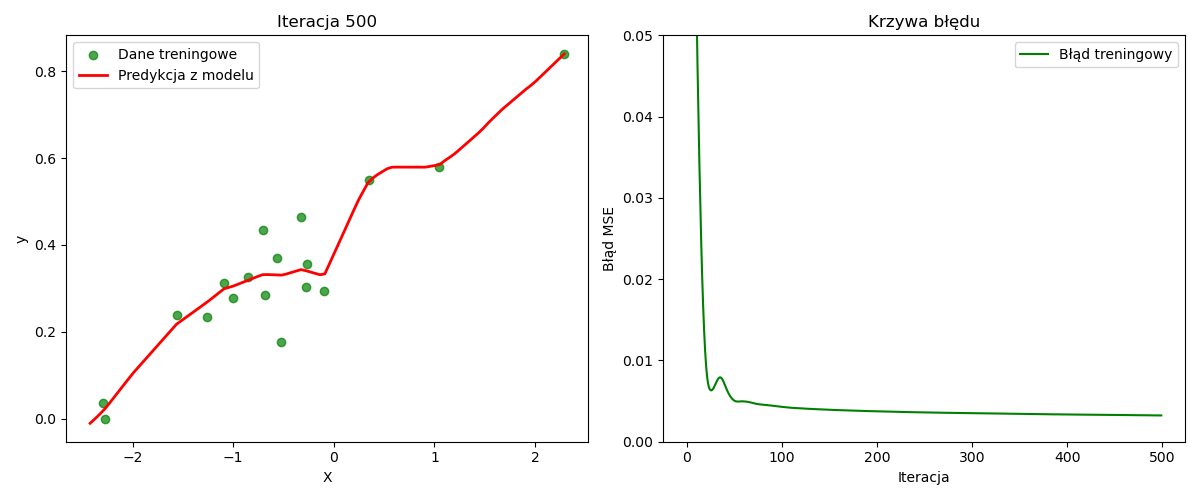
\includegraphics[width=\thiscaly\textwidth]{images/ot500False.png}\end{center}\end{frame}
\begin{frame}\begin{center}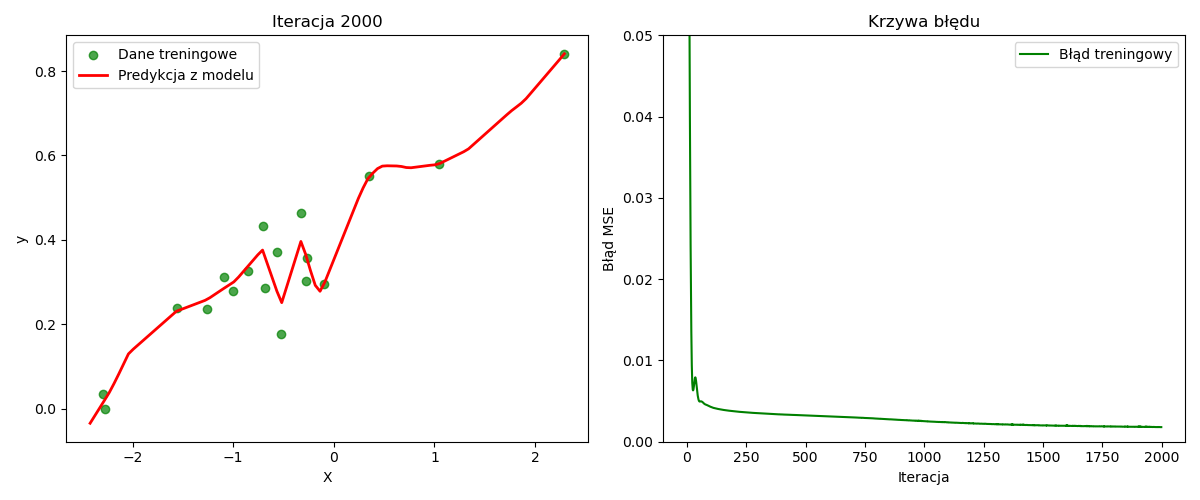
\includegraphics[width=\thiscaly\textwidth]{images/ot2000False.png}\end{center}\end{frame}

\begin{frame}\begin{center}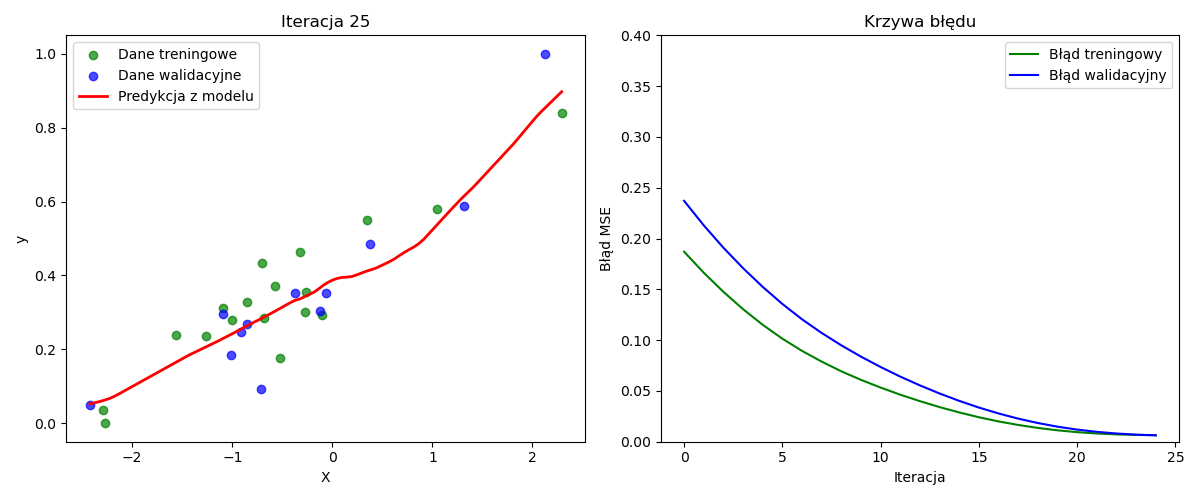
\includegraphics[width=\thiscaly\textwidth]{images/ot25True.png}\end{center}\end{frame}
\begin{frame}\begin{center}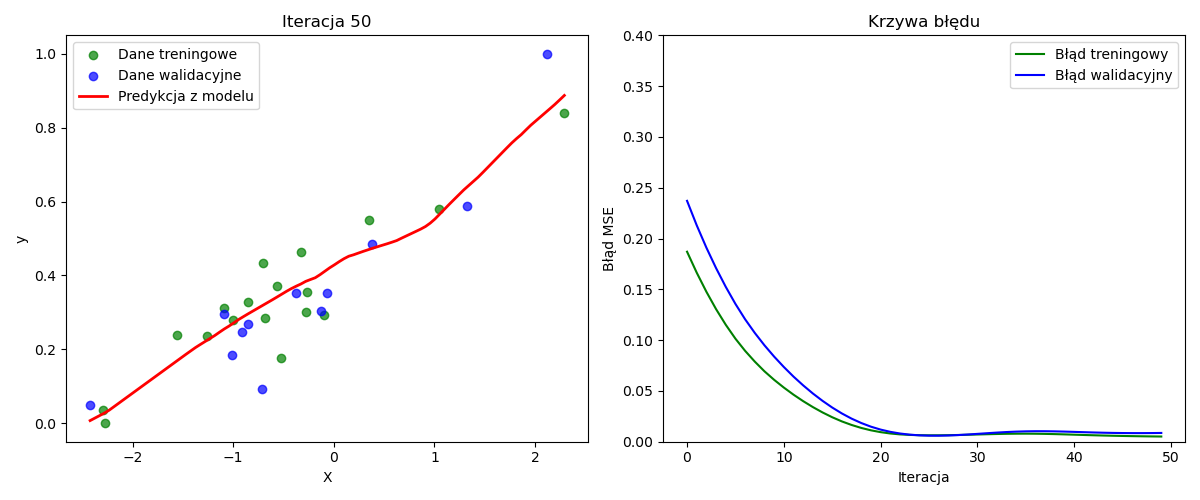
\includegraphics[width=\thiscaly\textwidth]{images/ot50True.png}\end{center}\end{frame}
\begin{frame}\begin{center}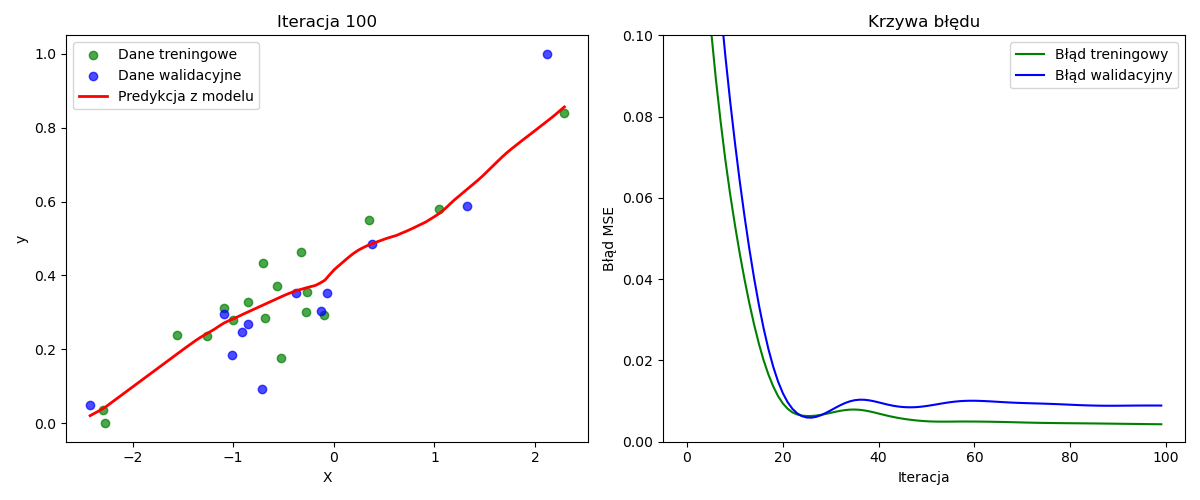
\includegraphics[width=\thiscaly\textwidth]{images/ot100True.png}\end{center}\end{frame}
\begin{frame}\begin{center}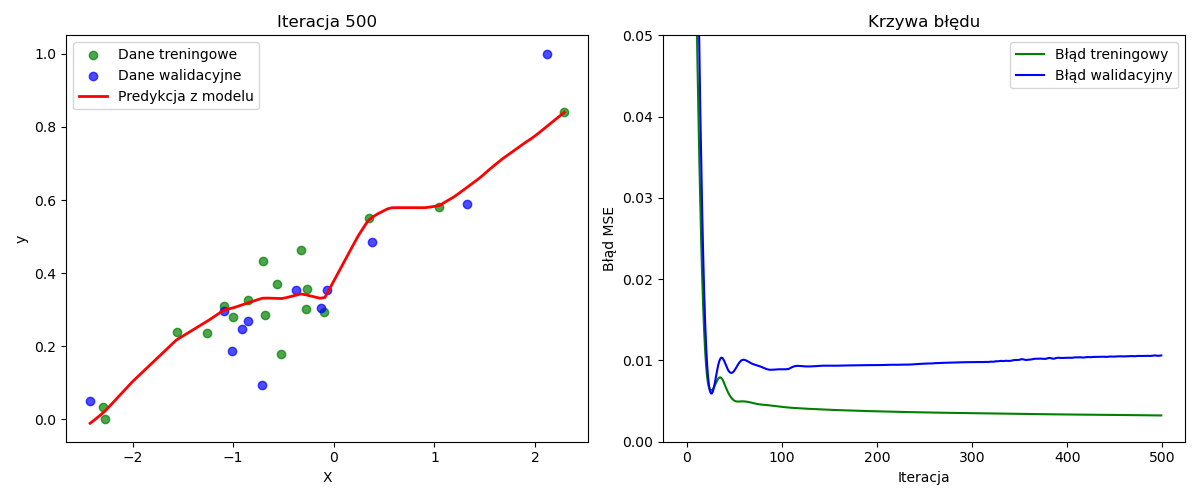
\includegraphics[width=\thiscaly\textwidth]{images/ot500True.png}\end{center}\end{frame}
\begin{frame}\begin{center}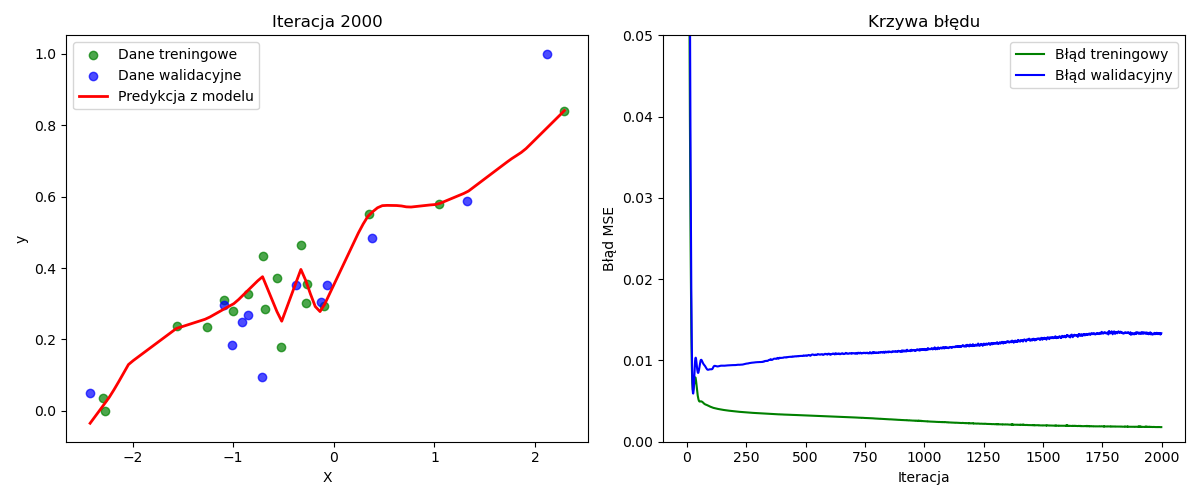
\includegraphics[width=\thiscaly\textwidth]{images/ot2000True.png}\end{center}\end{frame}

\begin{frame}
	\begin{description}
		\item[zbiór treningowy] optymalizacja wag modelu
		\item[zbiór walidacyjny] zabezpiecza przed przetrenowaniem, pozwala wybrać hiperparametry (np. learning rate 0.01 czy 0.001?), ułatwia decyzję o zakończeniu treningu, diagnostyka procesu treningu
		\item[zbiór testowy] oszacowanie rzeczywistej wydajności (skuteczności, wyniku) wytrenowanego modelu
	\end{description}
	\vskip 0.5 cm
	Zbiory rozłączne!
	\vskip 0.5 cm
	\begin{itemize}
		\item \textbf{Przetrenowanie} -- przesadne dopasowanie do zbioru treningowego
		\item \textbf{Generalizacja} -- dopasowanie do charakterystyki danych, którą zbiór treningowy reprezentuje
	\end{itemize}
\end{frame}

\begin{frame}
	Zmienne procesu treningu:
	\begin{enumerate}
		\item Dane
			\begin{enumerate}
				\item Rozmiar zbioru, liczba przykładów -- czy jest wystarczający?
				\item Diagnostyka przykładów -- podobieństwo/różnorodność? Outliery?
				%     Check your data against a data schema to detect bad examples, and then remove the bad examples from the training set. / The input data contains a burst of outliers. / The input data contains one or more NaNs—for example, a value caused by a division by zero.
			\end{enumerate}
		\item Model
			\begin{enumerate}
				\item Architekura -- liczba warstw, liczba neuronów
				\item Dobór hiperparametrów, regularyzacja
				\item Rozmiar modelu względem rozmiaru zbioru danych
			\end{enumerate}			
		\item Trening
			\begin{enumerate}
				\item Dostępne zasoby obliczeniowe -- przeszukiwanie przestrzeni hiperparametrów, sprawdzenie różnych stanów początkowych
				% Multiple random initializations can reduce the likelihood of being stuck in a bad local minimum, as the network starts optimization from different points.
				\item Weryfikacja zbieżności na podzbiorze przykładów 
				%     Reduce the training set to a tiny number of trustworthy examples. / Although this technique sounds artificial, it is actually a good idea. Assuming that the model converges on the small set of trustworthy examples, you can then gradually add more examples, perhaps discovering which examples cause the loss curve to oscillate.
				\item Diagnostyka wyników
			\end{enumerate}
	\end{enumerate}
\end{frame}


\begin{frame}
	Co jeżeli zbiór danych jest niewystarczający?\pause\ Augmentacja danych (\textbf{data augmentation})\pause
	\begin{itemize}
		\item Wprowadzenie szumu (różnego rodzaju)
		\item Edycja strukturalna (wycięcie fragmentu, obroty, skalowanie, \dots)
		\item Składanie nowego przykładu z kilku przykładów
		\item \dots
	\end{itemize}
	\begin{center}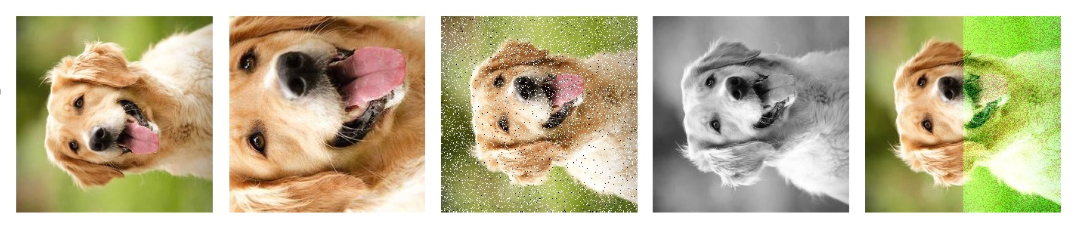
\includegraphics[width=0.67\textwidth]{images/aug.png}\end{center}
	{\tiny Źródło ilustracji: \href{https://arxiv.org/abs/2301.02830}{T. Kumar et al, Image Data Augmentation Approaches: A Comprehensive Survey and Future directions,  arXiv:2301.02830}}
\end{frame}


\section{Konstrukcja sieci}

\subsection{Softmax}

\begin{frame}
	$y_{11} = \max(20x - 10, 0)\quad y_{12} = \max(40x - 200, 0) \quad y_{21} = \max(y_{11} - y_{12}, 0)$\vskip 0.3 cm\pause
	Regresja -- otrzymujemy wartość liczbową -- jak dobry jest owoc w skali 0-10\vskip 0.3 cm\pause
	A podział na ,,dobry'' i ,,zły'' -- klasyfikacja?\vskip 0.3 cm\pause
	Modyfikacja wyjścia sieci, tak żeby na końcu
	\begin{itemize}
		\item $y_{21}$ wartość liczbowa określająca jak bardzo przykład należy do klasy ,,dobry''
		\item $y_{22}$ [\dots] do klasy ,,zły''
	\end{itemize}\vskip 0.3 cm\pause
	Problematyczne uczenie, bo np.
	\begin{itemize}
		\item  $y_{21} = 0.02, y_{22} = 0.6 \rightarrow$ ,,zły owoc''
		\item  $y_{21} = 1.7, y_{22} = 0.6 \rightarrow$ ,,dobry owoc''
	\end{itemize}
\end{frame}

\begin{frame}
	Softmax: $\sigma(\mathbf{y})_i = \frac{e^{y_i}}{\sum_{j=1}^N e^{y_j}}$\vskip 0.3 cm\pause
	
	$\mathbf{y}_a=\begin{bmatrix} 0.02, 0.6 \end{bmatrix}$\\
	$\sigma\left(\begin{bmatrix} 0.02, 0.6 \end{bmatrix}\right)_1 = \frac{e^{0.02}}{e^{0.02} + e^{0.6}}\approx 0.36$\\
	$\sigma\left(\begin{bmatrix} 0.02, 0.6 \end{bmatrix}\right)_2 = \frac{e^{0.6}}{e^{0.02} + e^{0.6}}\approx 0.64$\\
	$\sigma\left(\mathbf{y}_a\right) \approx \begin{bmatrix} 0.36, 0.64 \end{bmatrix}$\vskip 0.3 cm\pause
	
	$\mathbf{y}_b=\begin{bmatrix} 1.7, 0.6 \end{bmatrix}$\\
	$\sigma\left(\mathbf{y}_b\right) \approx \begin{bmatrix} 0.75, 0.25 \end{bmatrix}$	\vskip 0.3 cm
	Szacowane prawdopodobieństwo przynależności do poszczególnych klas
\end{frame}


\subsection{Funkcje aktywacji}


\begin{frame}\begin{center}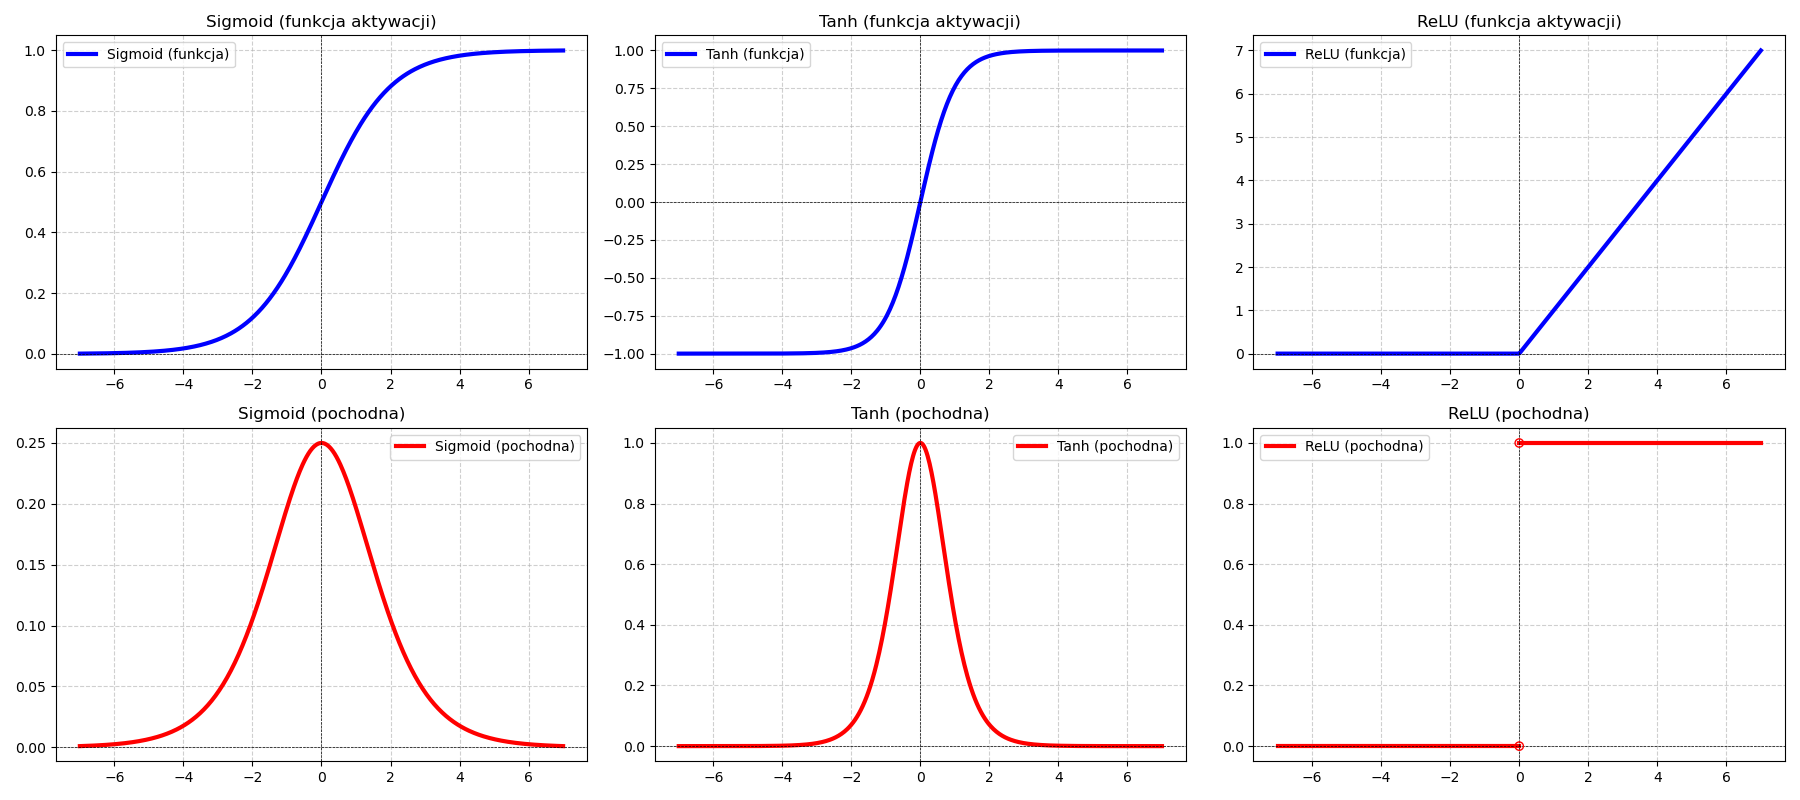
\includegraphics[width=\textwidth]{images/act.png}\end{center}\end{frame}
\begin{frame}[fragile]
Rozważmy zbiór danych (fragment zbioru Iris):
\begin{verbatim}
[[5.1 3.5 1.4 0.2]
 [4.9 3.  1.4 0.2]
 [4.7 3.2 1.3 0.2]
 [4.6 3.1 1.5 0.2]
 [5.  3.6 1.4 0.2]
 [5.4 3.9 1.7 0.4]
 [4.6 3.4 1.4 0.3]
 [5.  3.4 1.5 0.2]
 [4.4 2.9 1.4 0.2]
 [4.9 3.1 1.5 0.1]]	
\end{verbatim}
i neuron ReLU z wagami $\begin{bmatrix} 0.2, -0.4,  0.1, -0.5 \end{bmatrix} $\pause
\vskip 0.2 cm
$5.1 \times 0.2 + 3.5 \times -0.4 + 1.4 \times 0.1 + 0.2 \times -0.5 = 1.02 - 1.4 + 0.14 - 0.1 = -0.34$ \dots\\ \dots i tak dla każdego --
neuron jest ,,martwy'' (brak niezerowej wartości, zerowy gradient)
\end{frame}
\begin{frame}
	$\mathrm{ReLU}(x) = \max(x, 0)$
	\vskip 0.6 cm
	Alternatywy:
	\begin{itemize}
		\item Leaky ReLU $f(x) = \begin{cases} x & x > 0,\\ \alpha x & x \leq 0 \end{cases}$, np. $\alpha = 0.1$
		\item Parametric ReLU ($\alpha$ jest parametrem wyznaczanym w trakcie treningu)
		\item SiLU $f(x) = x \times \mathrm{sigmoid}(x)$
		\item ELU  $f(x) = \begin{cases} x & x > 0,\\ \alpha (e^x-1) & x \leq 0 \end{cases}$, $\alpha \geq 0$ jest hiperparametrem
		\item Softplus $f(x) = \ln(1 + e^x)$
		\item \dots
	\end{itemize}
\end{frame}


\subsection{Funkcje błędu (loss)}


\begin{frame}
	\begin{itemize}
		\item Mean Squared Error (MSE) $L(x,y) = (x - y)^2$
		\item Mean Absolute Error (MAE) $L(x,y) = |x - y|$
		\item Negative Log-Likelihood Loss function (NLL) $L(x,y) = -y\log x - (1 - y)\log (1 - x)$
		\item Cross-Entropy Loss ($\approx$ softmax + NLL)
		\item Margin Ranking Loss $L(x_1,x_2,y) = \max(0, -y(x_1 - x_2) + m)$, ($m$ margines)
		\item Kullback-Leibler Divergence Loss $L(x,y) = y(\log y - x)$
		\item \dots  
	\end{itemize}
\end{frame}


\subsection{Zaawansowane architektury -- sieci konwolucyjne}


\begin{frame}
	Problem: rozpoznawanie obiektów w obrazach
	\begin{itemize}
		\item Obiekt przesunięty, obrócony, przeskalowany, zdeformowany (operacja rzutowania)
		\item Cechy charakterystyczne -- złożone, rzadkie, różne dla różnych rodzajów obiektów
	\end{itemize}
\end{frame}
\begin{frame}
	Model HMAX:
	\begin{center}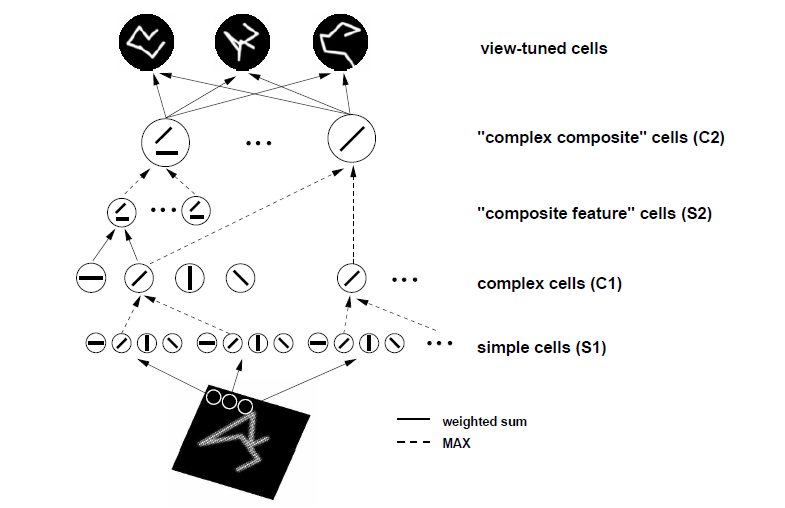
\includegraphics[width=0.67\textwidth]{images/hmax.png}\end{center}
	{\tiny Źródło ilustracji: Riesenhuber, M. \& Poggio, T. Hierarchical models of object recognition in cortex. Nat. Neurosci. 2, 1019-1025}
\end{frame}
\begin{frame}
	Architektura konwolucyjna:
	\begin{itemize}
		\item Filtry konwolucyjne (uczone/trenowane)
		\item Operacja ,,zbierania'' (pooling)
		\item Pary konwolucja+pooling powtórzone kilka razy
		\item Na końcu kilka warstw sieci MLP
	\end{itemize}
	\begin{center}\includegraphics[width=0.67\textwidth]{images/lenet5.png}\end{center}
	{\tiny Źródło ilustracji:  Lecun, Y.; Bottou, L.; Bengio, Y.; Haffner, P. (1998). "Gradient-based learning applied to document recognition" (PDF). Proceedings of the IEEE. 86 (11): 2278–2324}
\end{frame}
\begin{frame}
	\begin{center}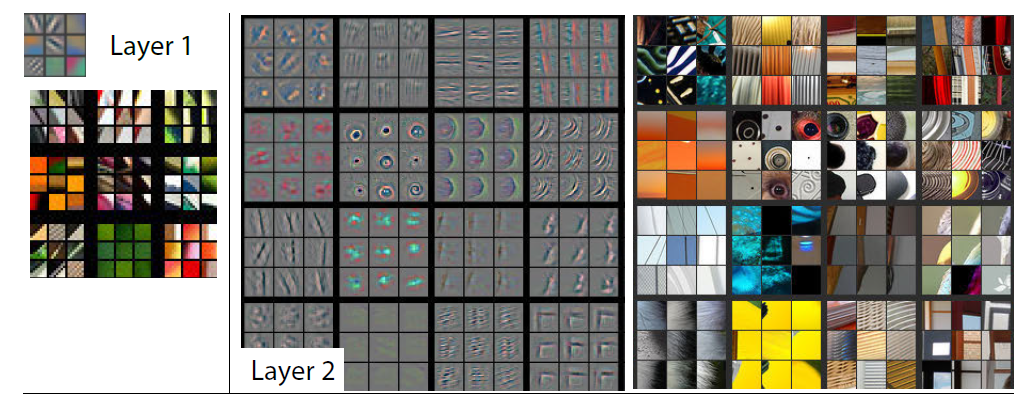
\includegraphics[width=0.67\textwidth]{images/layer12.png}\end{center}
	{\tiny Źródło ilustracji: Zeiler, M.D., Fergus, R. (2014). Visualizing and Understanding Convolutional Networks. In: Fleet, D., Pajdla, T., Schiele, B., Tuytelaars, T. (eds) Computer Vision – ECCV 2014}
\end{frame}
\begin{frame}
	\begin{center}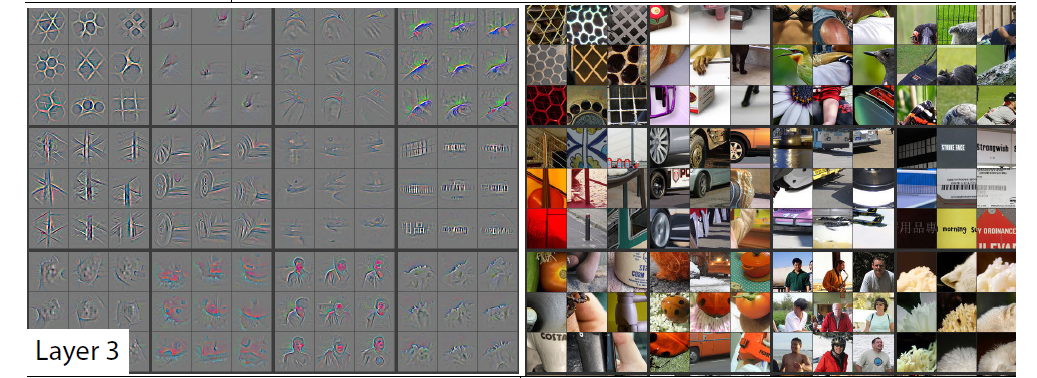
\includegraphics[width=0.67\textwidth]{images/layer3.png}\end{center}
	{\tiny Źródło ilustracji: Zeiler, M.D., Fergus, R. (2014). Visualizing and Understanding Convolutional Networks. In: Fleet, D., Pajdla, T., Schiele, B., Tuytelaars, T. (eds) Computer Vision – ECCV 2014}
\end{frame}
\begin{frame}
	\begin{center}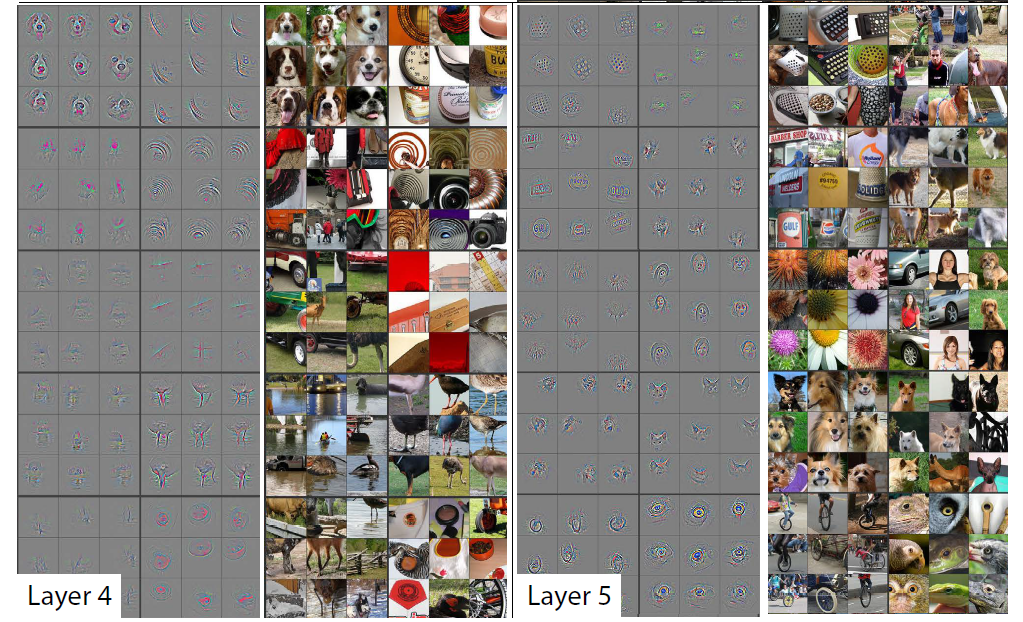
\includegraphics[width=0.67\textwidth]{images/layer45.png}\end{center}
	{\tiny Źródło ilustracji: Zeiler, M.D., Fergus, R. (2014). Visualizing and Understanding Convolutional Networks. In: Fleet, D., Pajdla, T., Schiele, B., Tuytelaars, T. (eds) Computer Vision – ECCV 2014}
\end{frame}
\begin{frame}
	Sieci ResNet
	\begin{center}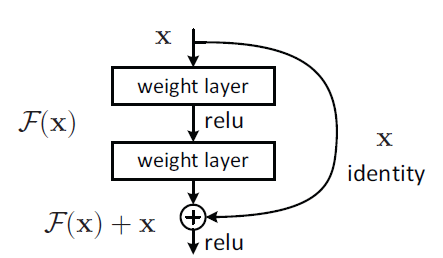
\includegraphics[width=0.2\textwidth]{images/rblock.png}\end{center}
	\begin{center}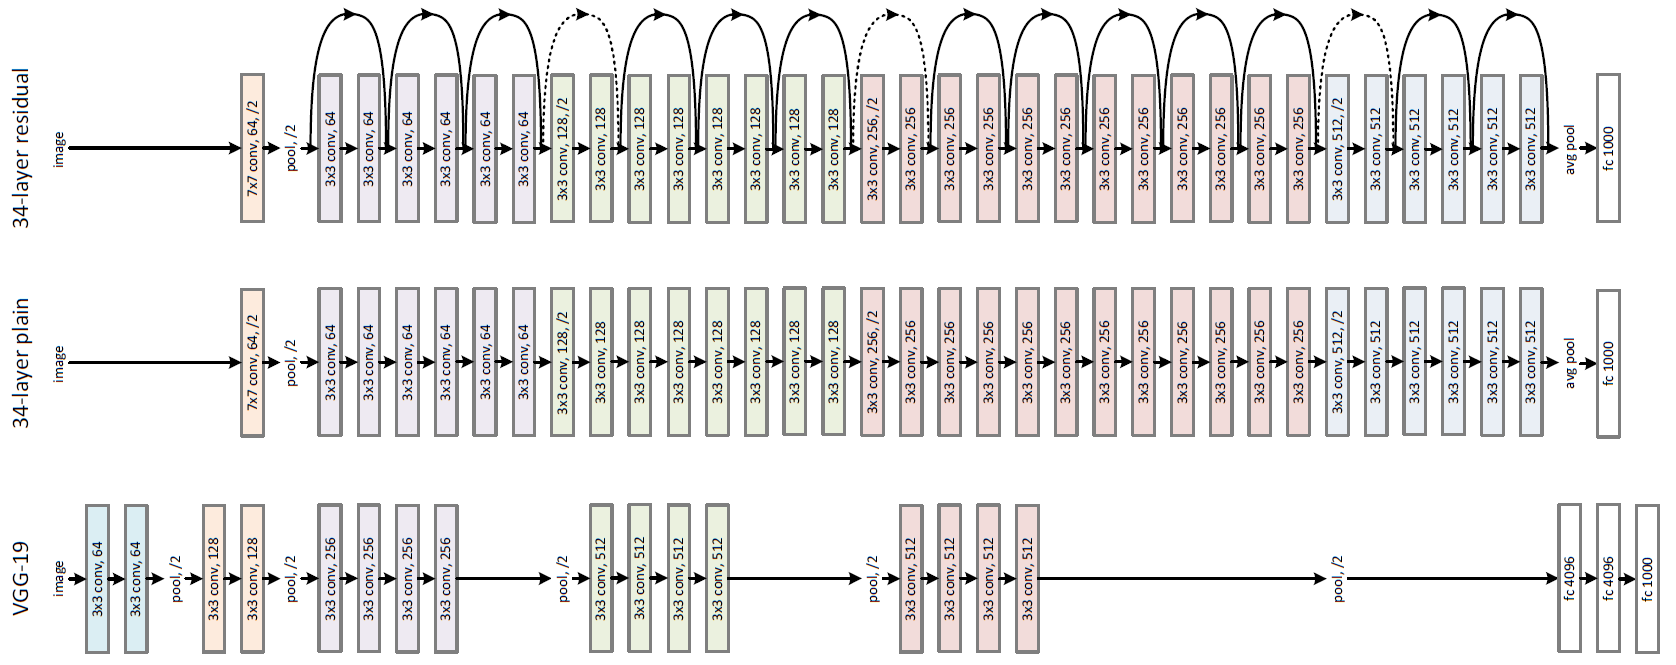
\includegraphics[width=0.6\textwidth]{images/resnet.png}\end{center}
	{\tiny Źródło ilustracji: K. He, X. Zhang, S. Ren and J. Sun, "Deep Residual Learning for Image Recognition," 2016 IEEE Conference on Computer Vision and Pattern Recognition (CVPR), 2016, pp. 770-778}
\end{frame}


\subsection{Zaawansowane architektury -- sieci transformers}


\begin{frame}
	\begin{center}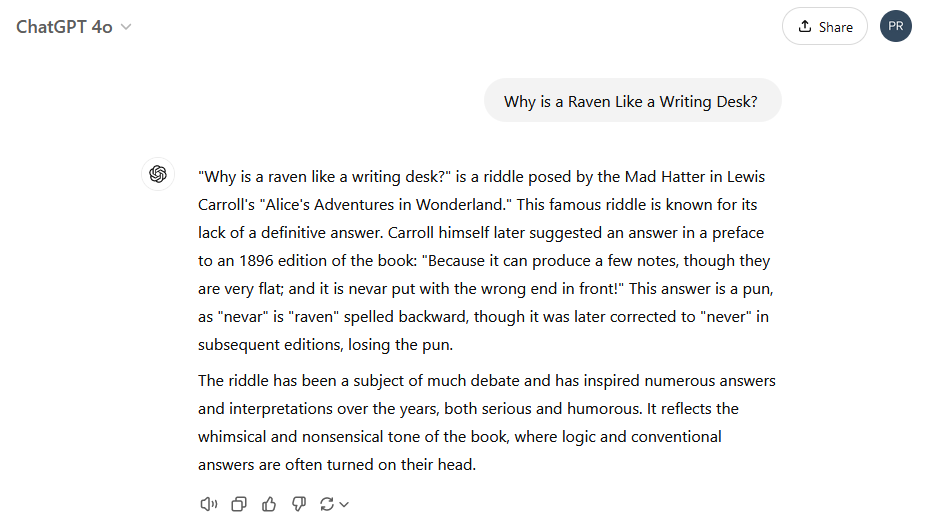
\includegraphics[width=0.8\textwidth]{images/raven.png}\end{center}
\end{frame}
\begin{frame}[fragile]
Problem ,,sekwencja w sekwencję'' (sequence to sequence), z odległymi zależnościami między słowami
\begin{verbatim}
                 Mary had a little lamb.
In the hospital, Mary had a little lamb.
\end{verbatim}
\vskip 1cm
Krótka (i fragmentaryczna) historia prób rozwiązania:
\begin{itemize}
	\item Sieci rekurencyjne
	\item Sieci LSTM (Long-Short Term Memory)
	\item Sieci transformers
\end{itemize}
\end{frame}
\begin{frame}
	\begin{center}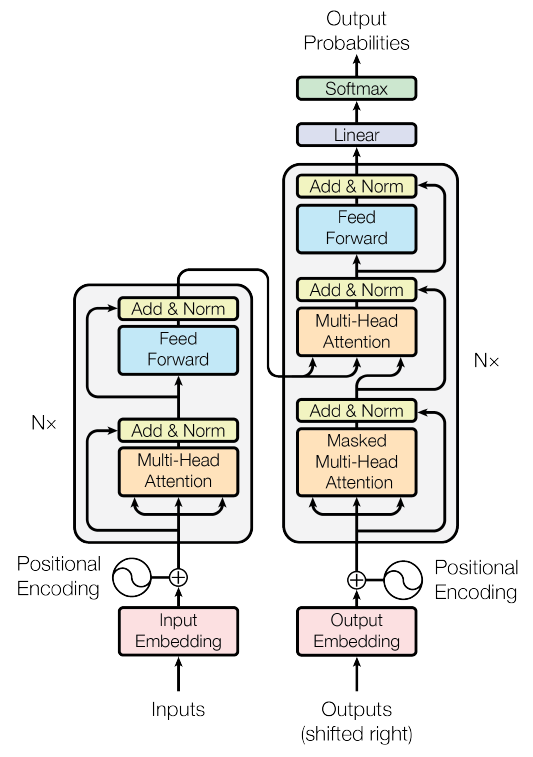
\includegraphics[width=0.33\textwidth]{images/att.png}\end{center}
	{\tiny Źródło ilustracji: Vaswani, A. et al (2017). "Attention is All you Need". Advances in Neural Information Processing Systems. 30}
\end{frame}
\begin{frame}
	$\mathrm{Attention}(Q, K, V) = \mathrm{softmax}\left(\frac{QK^\top}{\sqrt{d_k}}\right)V$
	\begin{center}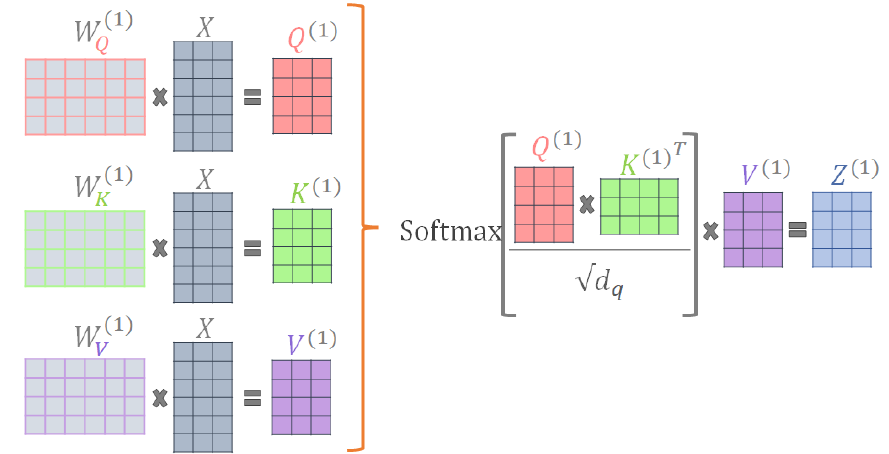
\includegraphics[width=0.6\textwidth]{images/attsee.png}\end{center}
	{\tiny Źródło ilustracji: Ahmed, S., Nielsen, I.E., Tripathi, A. et al. Transformers in Time-Series Analysis: A Tutorial. Circuits Syst Signal Process 42, 7433-7466 (2023)}
\end{frame}
\begin{frame}
	\begin{center}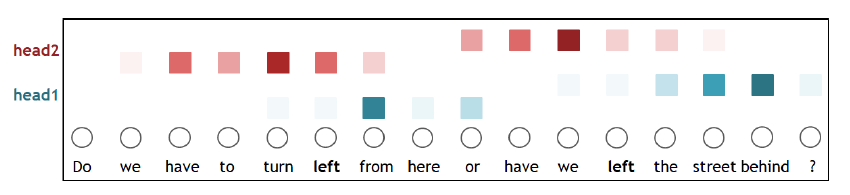
\includegraphics[width=0.8\textwidth]{images/left.png}\end{center}
	{\tiny Źródło ilustracji: Ahmed, S., Nielsen, I.E., Tripathi, A. et al. Transformers in Time-Series Analysis: A Tutorial. Circuits Syst Signal Process 42, 7433-7466 (2023)}
\end{frame}



\end{document}

